\chapter{Исследование производительности систем радиочастотной идентификации}\label{ch:ch2}

В настоящей главе исследуется возможность использования технологии пассивной радиочастотной идентификации стандарта EPC Gen-2 \cite{StdGen2} для идентификации автотранспорта, движущегося со скоростями порядка 60 "--- 150 км/ч. Сначала, в разделе \ref{sec:ch2_structure}, будут описаны компоненты системы радиочастотной идентификации автомобилей, а в разделе \ref{sec:ch2_general_scheme} также в наиболее общей форме приведены зависимости, определяющие вероятность успешной идентификации подвижной метки. Эта вероятность зависит от числа раундов, в которых метка успевает принять участие, а также от вероятности идентификации в каждом из раундов. Для анализа факторов, от которых зависит число раундов, в разделе \ref{sec:ch2_durations} будут исследованы зависимости длительностей команд, ответов и раундов от различных параметров протокола, а для анализа вероятности идентификации метки в каждом из раундов в разделе \ref{sec:ch2_channel} будет приведена модель радиоканала, учитывающая особенности многолучевого распространения сигналов вблизи дороги, зависимость мощности отраженных сигналов от материала поверхности дороги, а также влияние эффекта Доплера, и будут получены оценки вероятностей битовых ошибок (BER) при передаче ответов меток. С учетом сделанных расчетов будет уточнено определение области, в которой метки имеют возможность передать свои идентификаторы считывателю, и будет сделан аналитический расчет вероятности идентификации метки. В разделе \ref{sec:ch2_results} кратко описывается имитационная модель и приводятся результаты моделирования системы радиочастотной идентификации автомобилей. Раздел \ref{sec:ch2_conclusion} завершает главу. В следующей главе будет приведена аналитическая модель, позволяющая более точно оценить влияние сбросов питания и смены флагов опроса на вероятность идентификации.

Результаты, представленные в главе, были опубликованы в журналах \cite{RFID_JRFID2017,QS_TCOMM2012,QS_JITCS2013}, сборниках, индексируемых Scopus/WoS \cite{RFID_IEEERFID2017,RFID_DCCN2016_CCIS,RFID_SYNCHROINFO2018}, и представлены в трудах конференций \cite{Fedotov2020, Fedotov2020a, RFID_DCCN2015_RUS,RFID_DCCN2013_RUS}.





%%%%%%%%%%%%%%%%%%%%%%%%%%%%%%%%%%%%%%%%%%%%%%%%%%%%%%%%%%%%%%%%%%%%%%%%%%%%%%%%
\section{Структура системы радиочастотной идентификации} \label{sec:ch2_structure}
%%%%%%%%%%%%%%%%%%%%%%%%%%%%%%%%%%%%%%%%%%%%%%%%%%%%%%%%%%%%%%%%%%%%%%%%%%%%%%%%
Система радиочастотной идентификации автомобилей состоит из RFID-считывателя и RFID-меток (радиометок), размещенных на автомобилях (см. рис.~\ref{fig:ch2_system_structure}). Метки и считыватель работают по стандарту EPC Class 1 Generation 2 \cite{StdGen2}

\begin{figure}[ht]
  \centerfloat{
    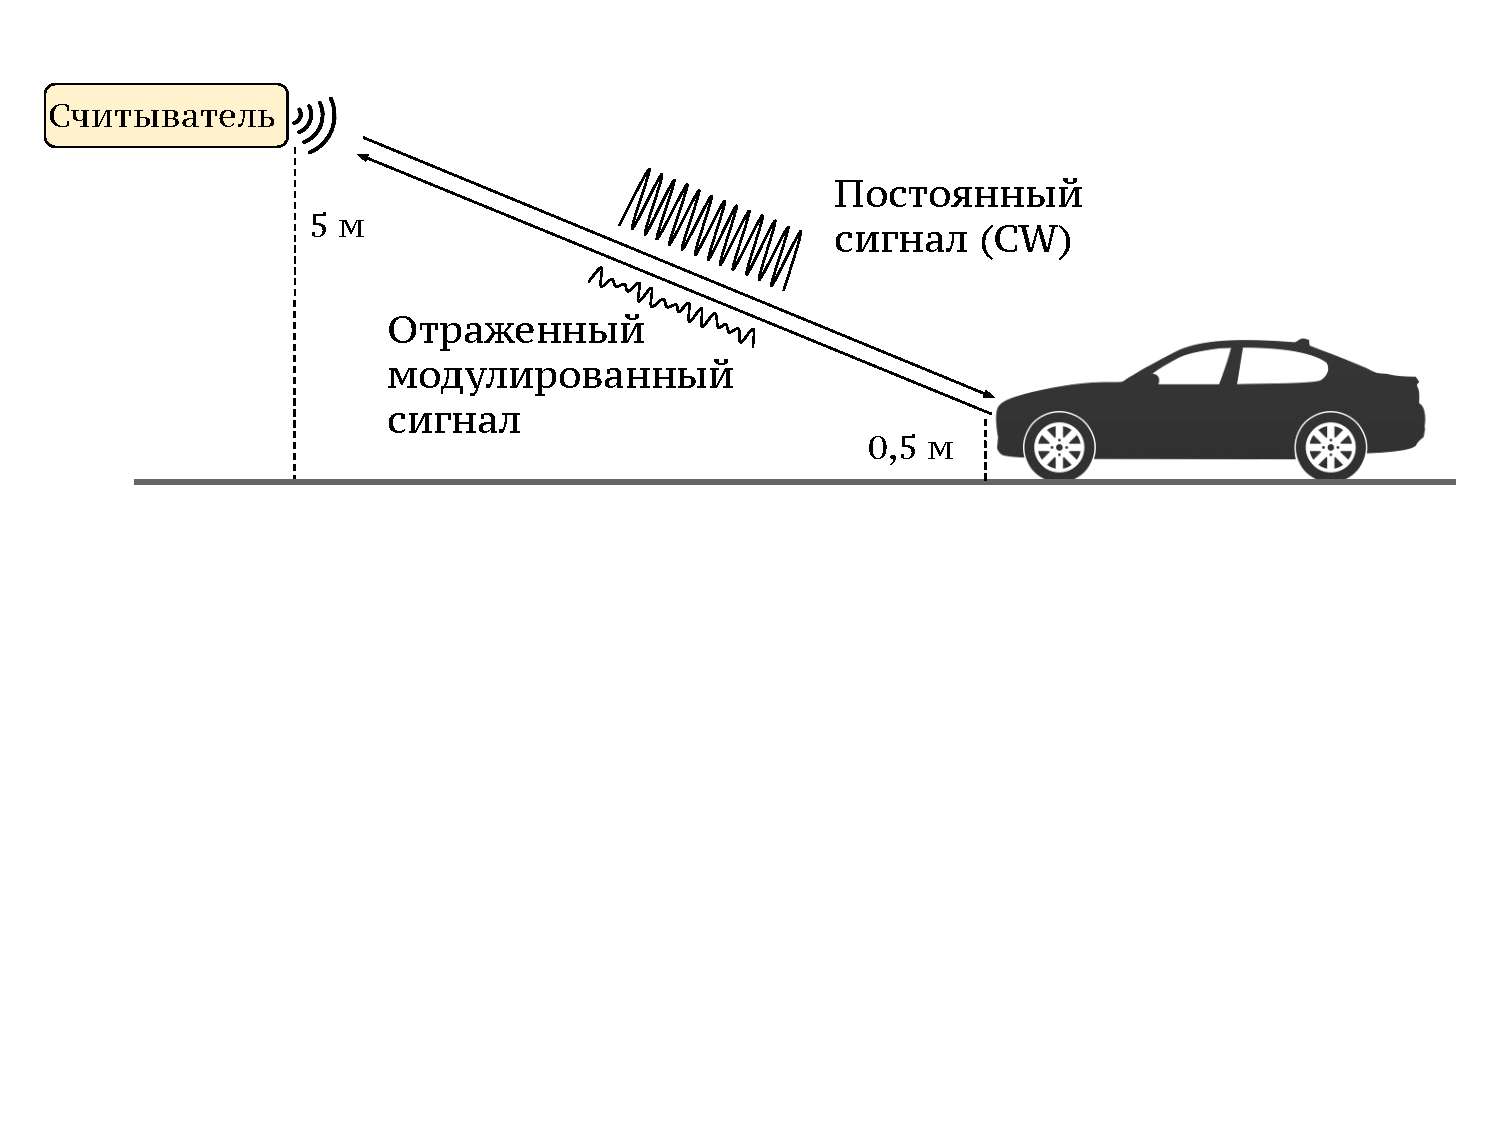
\includegraphics [scale=0.5] {chapter2/ch2_system_structure}
  }
  \caption{Структура системы радиочастотной идентификации автомобилей}
  \label{fig:ch2_system_structure}
\end{figure}

Метки могут размещаться на регистрационных номерных знаках, под лобовым стеклом или на корпусе автомобиля. В настоящей работе рассматривается случай, когда метки расположены на номерах, поскольку этот вариант был использован в проведенном в г. Казань эксперименте. Кроме того, размещение меток в номерных знаках обладает рядом преимуществ: расположение знаков относительно дорожного полотна варьируется в малых пределах, зона номерного знака не загорожена никакими проводящими поверхностями, наконец это решение можно в дальнейшем легко стандартизировать и масштабировать за счет монтирования меток в выпускаемые номерные знаки.

RFID-считыватель размещается над дорогой (например, на тех же опорах, на которых сегодня размещаются камеры), на высоте приблизительно 5 метров; считыватель может оснащаться от 1 до 4 антенн. Таким образом, один считыватель может читать метки в передних и задних номерах на двухполосной дороге.

Связь между меткой и считывателем возможна при соблюдении двух условий: метка получает достаточно энергии для работы и декодирования команд от считывателя (чувствительность современных меток имеет порядок -18 дБм), и отраженный модулированный меткой сигнал поступает на считыватель на достаточно высокой мощности, чтобы быть успешно распознанным и декодированным (при отсутствии коллизий, уровень принимаемого сигнала для современных считывателей должен быть не ниже минус 80 дБм). На практике это означает, что дальность связи составляет порядка 8 -- 15 метров. Однако, из-за особенностей распространения сигнала вблизи автодороги, область, в которой метка может получить достаточно энергии, может иметь достаточно сложный вид и состоять из нескольких непересекающихся областей, общая ширина которых может составлять 2 -- 3 метра. Подробнее эти эффекты будут рассмотрены в последующих разделах.



%%%%%%%%%%%%%%%%%%%%%%%%%%%%%%%%%%%%%%%%%%%%%%%%%%%%%%%%%%%%%%%%%%%%%%%%%%%%%%%%
\section{Общая схема расчёта вероятности идентификации автомобилей}\label{sec:ch2_general_scheme}
%%%%%%%%%%%%%%%%%%%%%%%%%%%%%%%%%%%%%%%%%%%%%%%%%%%%%%%%%%%%%%%%%%%%%%%%%%%%%%%%
Производительность системы определяется как доля успешно идентифицированных автомобилей. Полагая, что успешного чтения хотя бы одной метки достаточно для идентификации автомобиля, вероятность идентификации можно описать следующим образом:

$$
	\mathbb{P}\{A_x\} = 1 - \prod\limits_{\forall t \in  \mathfrak{T}_x} (1 - \mathbb{P}\{A_t\}),
$$
где $A_x$ "--- событие идентификации автомобиля $x$, $A_t$ "--- событие идентификации метки $t$, а $\mathfrak{T}_x$ есть множество меток, размещенных на автомобиле $x$. Вероятность идентификации метки $\mathbb{P}\{A_t\}$ зависит от длительности раунда инвентаризации, вероятности успешной передачи ответа и числа меток в области чтения:

$$
	\mathbb{P}\{A_t\} = 1 - (1 - (1 - \mathbb{P}\{A_c\})\mathbb{P}\{A_r\})^{N_r},
$$
где $A_c$ "--- событие возникновения коллизии, $A_r$ "--- событие успешной передачи меткой ее идентификатора и $N_r$ "--- число раундов, в которых метка успевает принять участие.

Пусть $N_t$ "--- число меток в области чтения и $Q$ "--- параметр антиколлизионного протокола. \cite{StdGen2}. Тогда вероятность возникновения коллизии для данной метки определяется следующей формулой:

$$
	\mathbb{P}\{A_c\} = 1 - (1 - 2^{-Q})^{|N_t| - 1}.
$$

Число раундов можно грубо оценить как:

$$
	N_r \approx \frac{L}{v}\cdot\frac{1}{\tau},
$$
где $L$ "--- общая длина участка дороги с хорошими условиями для чтения (т.е. на этом участке метка получает достаточно энергии для работы и битовая ошибка достаточно низка), $\tau$ "--- средняя длина раунда при заданном числе меток и параметрах протокола, $v$ "--- скорость движения метки. В действительности количество раундов представлеяет собой случайную величину, зависящую от множества параметров, включая количество меток в области чтения, настройки протокола, непосредственный выбор метками слотов для ответов (определяет количество коллизий, пустых слотов и слотов с ответами). Также число раундов зависит от результатов попыток передачи меткой её идентификатора, а также от того, сбрасывал ли считыватель питание между раундами "--- влияние этих факторов оказывается очень существенным и исследуется подробнее в следующей главе диссертации.

Согласно \cite{Nikitin2008}, при отсутствии коллизий основным источником ошибок при расчете $\mathbb{P}\{A_r\}$ является высокий BER при приеме ответов от меток. Пусть $r$ "--- ответ метки, $\mathfrak{R}$ "--- множество всех ответов метки, передача которых необходима для успешной идентификации. Обозначая битовую длину ответа как $|r|$, вероятность успешной передачи всех ответов $\mathbb{P}\{A_r\}$ метки можно вычислить по формуле:

$$
	\mathbb{P}\{A_r\}=\prod_{r \in \mathfrak{R}}(1-B)^{|r|}.
$$

Множество $\mathfrak{R}$ обязательно содержит ответ RN16 на команду, с которой начался слот, в котором метка передаёт ответ (Query, QueryRep или QueryAdjust) и ответ на команду ACK (PC+EPC+CRC). Если для идентификации метки также используется 64-битное значение из банка TID, то $\mathfrak{R}$ также включает ответы на Req\_RN и Read.

Из приведенных формул видно, что для максимизации вероятности идентификации автомобиля необходимо увеличивать вероятность успешной передачи меткой ответов и число раундов, и одновременно уменьшать вероятность коллизий. Однако эти требования вступают в противоречие: более низкий BER достигается при более надежных и медленных настройках протокола, а вероятность коллизии снижается при росте числа слотов, но все это ведет к увеличению длительности раунда. В последующих разделах будет разработан комплекс моделей, позволяющий проанализировать вероятность идентификации метки при различных допущениях, а в конце главы будут приведены результаты расчета вероятности идентификации автомобиля при различных настройках протокола и скорости движения, полученные с помощью детализированной имитационной модели.







%%%%%%%%%%%%%%%%%%%%%%%%%%%%%%%%%%%%%%%%%%%%%%%%%%%%%%%%%%%%%%%%%%%%%%%%%%%%%%%%
\section{Анализ влияния параметров протокола на длительности раундов}\label{sec:ch2_durations}
%%%%%%%%%%%%%%%%%%%%%%%%%%%%%%%%%%%%%%%%%%%%%%%%%%%%%%%%%%%%%%%%%%%%%%%%%%%%%%%%
Считыватель использует модуляции DSB-ASK, SSB-ASK и PR-ASK, а в качестве схемы кодирования используется PIE. Из-за использования PIE (Pulse Interval Encoding) длительность передачи команды зависит от её содержания, так как длительности символов data\_0 и data\_1 отличаются в 1,5--2 раза. Перед каждой командой Query считыватель передает преамбулу, а перед остальными "--- более короткую синхронизирующую последовательность.

\begin{figure}[h]
	\centerfloat{
	  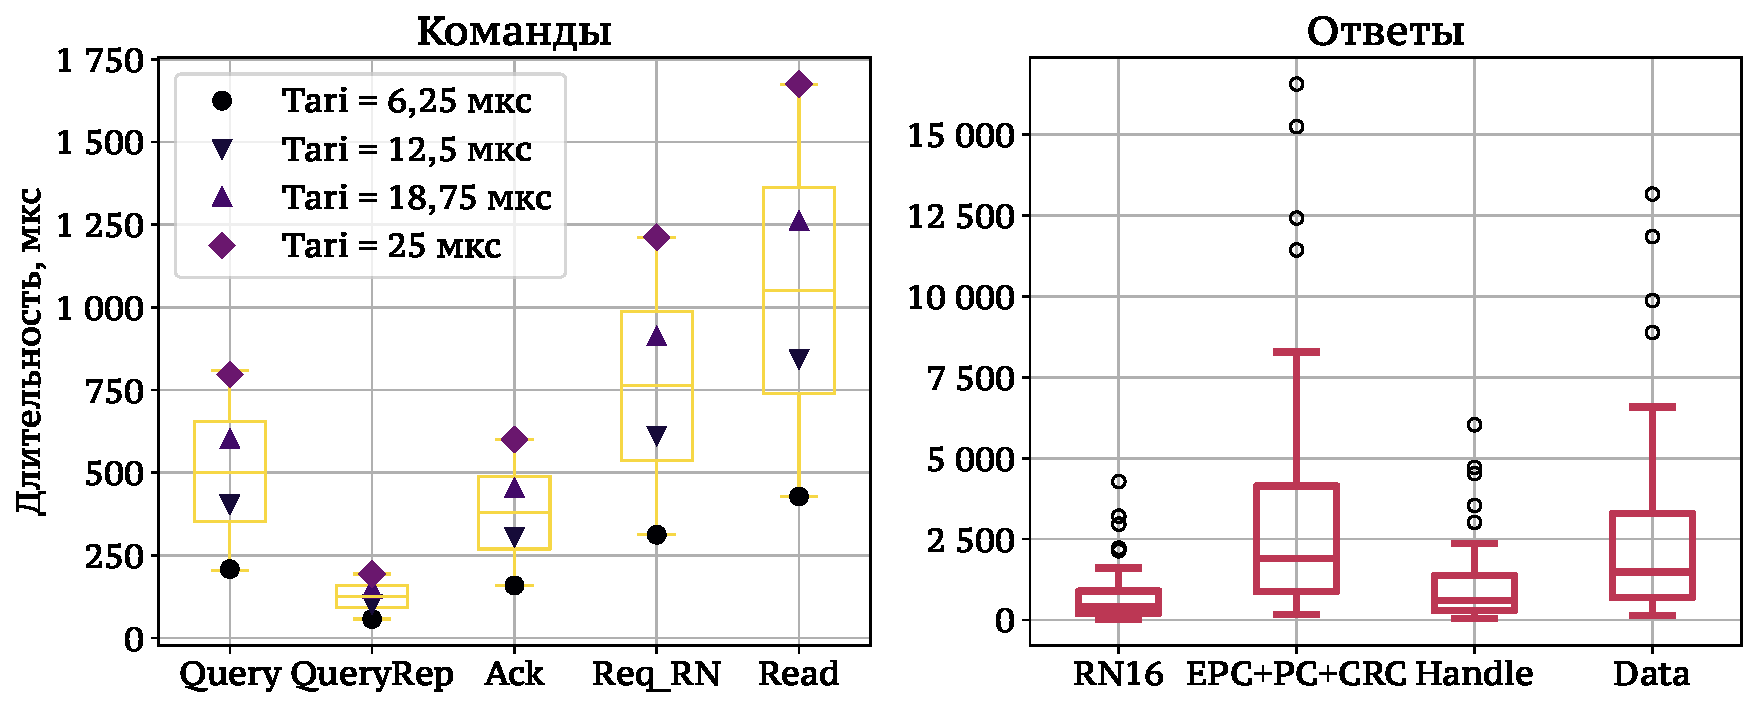
\includegraphics[width=0.9\textwidth]{chapter2/ch2_messages_durations}
	}
	\caption{Разброс длительностей сообщений между считывателем и меткой.}
	\label{fig:ch2_messages_durations}
\end{figure}

На рис.~\ref{fig:ch2_messages_durations} показан разброс длительностей команд считывателя и ответов меток для разных настроек протокола. Длительности команд могут различаться в четыре раза, так как все символы, передаваемые считывателем, пропорциональны длительности Tari. В действительности разброс длительностей команд еще больше "--- при построении графика предполагалось, что отношение длительностей RTcal, TRcal и Tari фиксировано ($\text{RTcal} = 2,75\;\text{Tari}$, $\text{TRcal} = 2,05\;\text{RTcal}$), а стандарт определяет их в диапазоне $2,5\;\text{Tari} \leqslant \text{RTcal} \leqslant 3\;\text{Tari}$ и $1,1\;\text{RTcal} \leqslant \text{TRcal} \leqslant 3\;\text{RTcal}$.

\begin{figure}[h]
	\centerfloat{
	  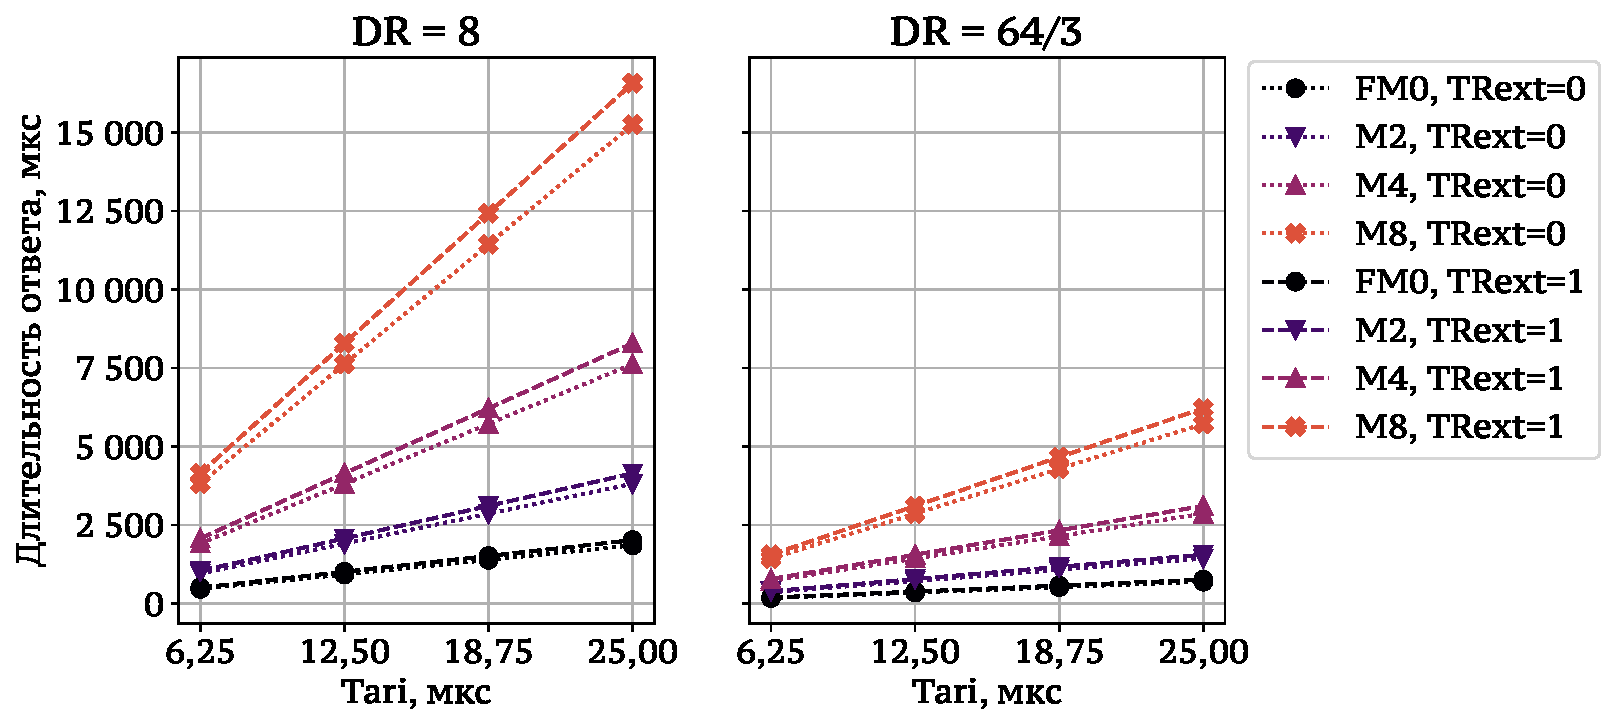
\includegraphics[width=0.9\textwidth]{chapter2/ch2_response_durations}
	}
	\caption{Зависимость длительностей ответов EPC+PC+CRC от параметров протокола.}
	\label{fig:ch2_response_durations}
\end{figure}

Разброс длительностей ответов меток даже больше, чем разброс длительностей команд. Это обусловлено тем, что длительности ответов зависят не только от Tari, но и от параметра DR, способа кодирования ответа (1, 2, 4 или 8 символов на бит) и того, используется ли расширешнная преамбула. На рис.~\ref{fig:ch2_response_durations} показаны зависимости длительностей ответов меток с передачей EPCID, PC и CRC от различных параметров протокола, полученные при фиксированном отношении Tari, RTcal и TRcal. Можно видеть, что, длительность ответа может меняться на два порядка.

При идентификации метки может использоваться только EPCID или комбинация EPCID и значений из других банков, например "--- TID. Первый вариант менее надежен, однако существенно быстрее второго "--- на чтение банков памяти требуется значительно больше времени, так как при этом необходимо осуществить дополнительный обмен сообщениями. На длительность идентификации также влияет, например, использование команды Select для настройки флагов меток и выбора подмножества меток для опроса. В дальнейшем будем рассматривать два самых простых сценария: идентификацию меток только по EPCID (в этом случае взаимодействие ограничивается инвентаризацией) и по комбинации EPCID + TID. Кроме того, будем предполагать, что считыватель не использует команды QueryAdjust и не изменяет выбранное значение параметра Q.

\begin{figure}[!t]
	\centerfloat{
	  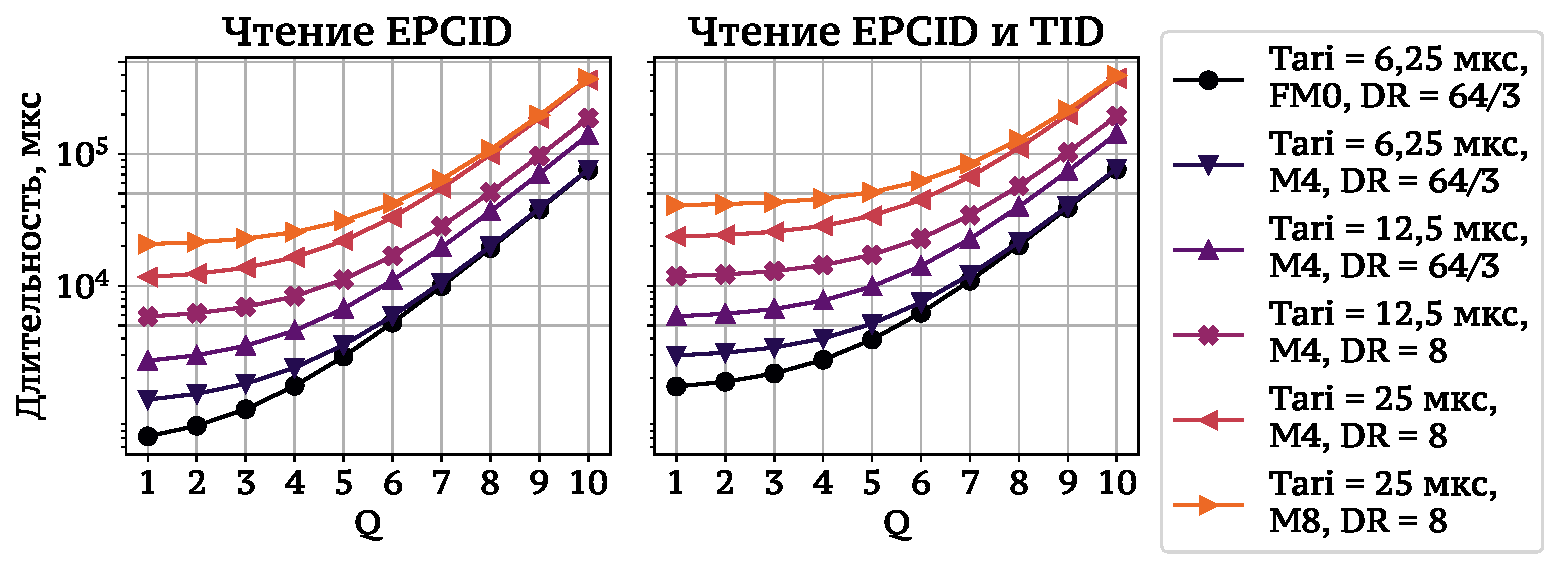
\includegraphics[width=0.9\textwidth]{chapter2/ch2_round_durations}
	}
	\caption{Зависимость максимальной длительности раунда от значения Q.}
	\label{fig:ch2_round_durations}
\end{figure}


Из-за ошибок при передаче ответов, в общем случае метке может потребоваться несколько попыток для передачи своего идентификатора. Максимальное число раундов, в которых может принять участие метка, ограничено областью, в которой она получает достаточно энергии, и скоростью ее движения. Более подробно число раундов, с учетом коллизий и ошибок, анализируется в главе 3, а сейчас рассмотрим простейший модельный случай, когда в раунде передачу ведет единственная метка, и ей удается передать все свои сообщения. То есть в раунде нет коллизий, а ошибки при передаче ответов если и происходят, то только на последних ответах. Длительность раунда $\tau$ для этого модельного случая можно рассчитать по формуле (см. рис.~\ref{fig:ch1_inventory}):

$$
	\tau = t_1 + (2^Q - 1) t_0,
$$
где
$$
	\begin{aligned}
		&t_0 = T_{\text{QueryRep}} + T_1 + T_3\;\text{ "--- пустой слот}\\
		&t_1 = \begin{cases}
			t_1^{\text{(epc)}} &\text{ "--- слот с ответом при идентификации по EPCID}\\
			t_1^{\text{(tid)}} &\text{ "--- слот с ответом при идентификации по EPCID и TID}
		\end{cases},\\
		&t_1^{\text{(epc)}} = T_{\text{Query}} + 2 * (T_1 + T_2) + T_{\text{RN16}} +
			T_{\text{ACK}} + T_{\text{EPCID}}\\
		&t_1^{\text{(tid)}} = t_1^{\text{(epc)}} + 2 * (T_1 + T_2) + T_{\text{Req\_RN}} +
			T_{\text{Handle} + T_{\text{Read}}} + T_{\text{Data}}
	\end{aligned}
$$
Здесь $T_1$ "--- интервал между концом команды и началом ответа, $T_2$ "--- интервал между концом ответа и следующей командой, $T_3$ "--- интервал между окончанием $T_1$ и новой командой (ожидание ответа), а $T_{\text{msg}}$ "--- длительность команды или ответа msg. Для простоты не учитываем задержку распространения сигнала, которая из-за небольшого расстояния крайне мала. На рис.~\ref{fig:ch2_round_durations} показаны зависимости длительностей раундов, рассчитанные по этим формулам, от значения Tari и величины Q.

\begin{figure}[h]
	\centerfloat{
		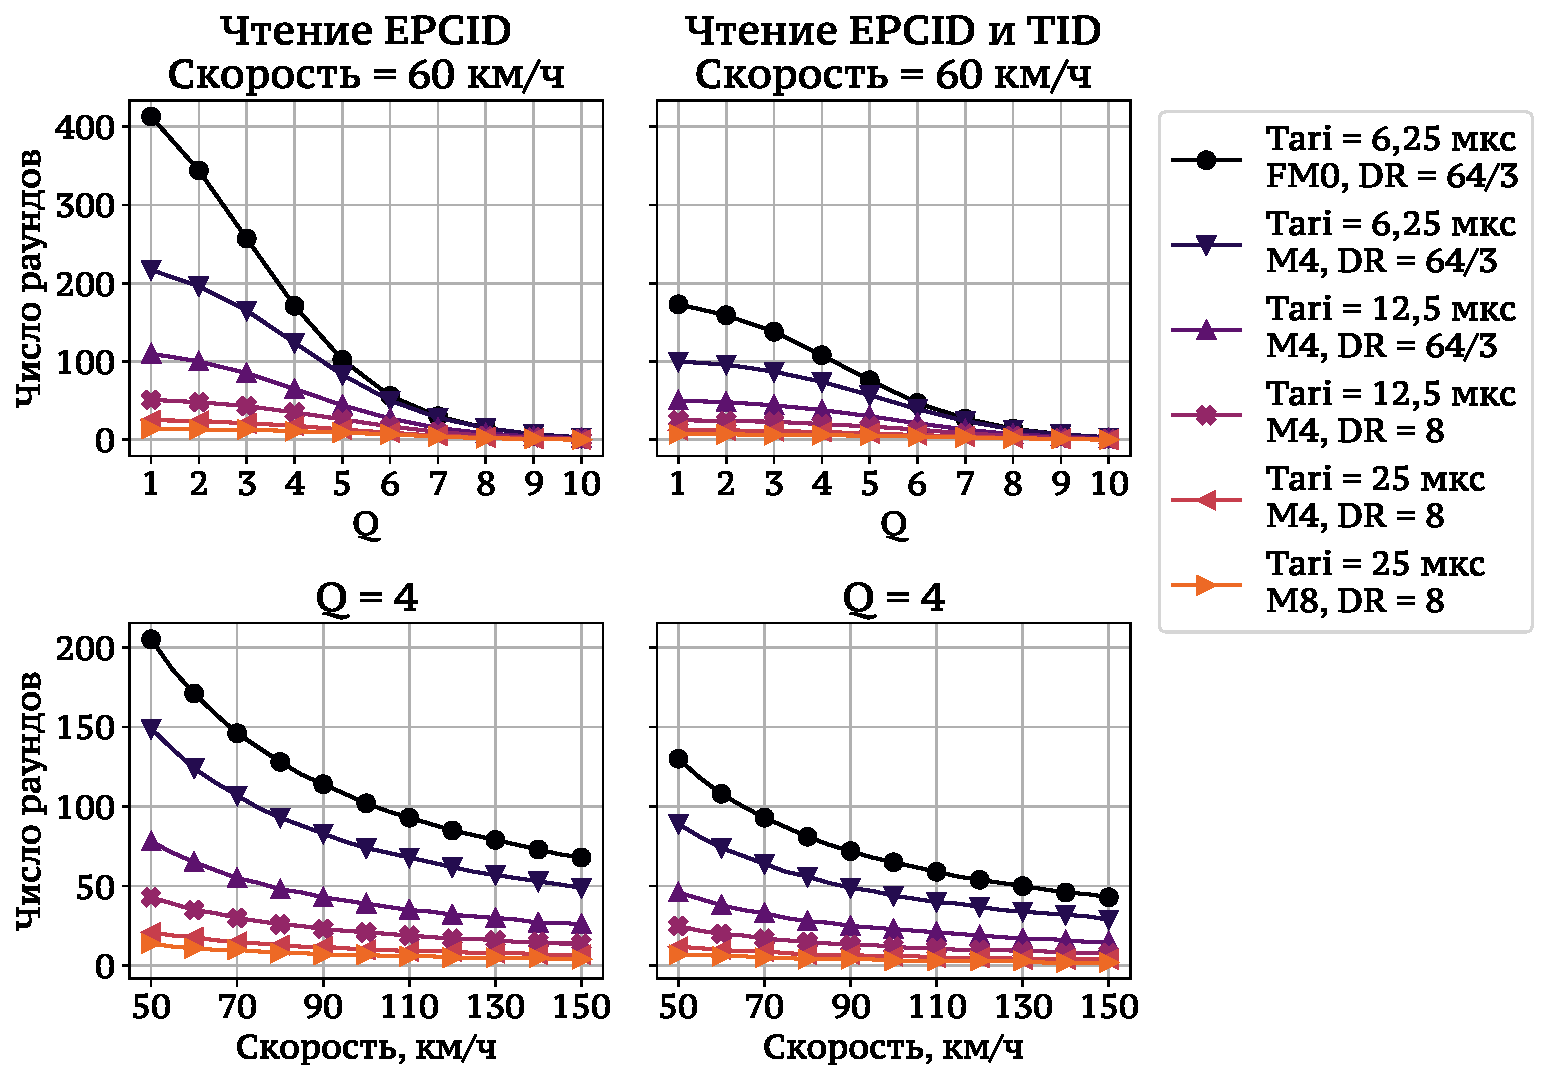
\includegraphics[width=0.9\textwidth]{chapter2/ch2_max_num_rounds.pdf}
	}
	\caption{Зависимость максимального числа раундов, в которых принимает участние метка, от значения Q.}
	\label{fig:ch2_max_num_rounds}
\end{figure}

Зная длительность раунда, скорость движения метки $v$ и размер $L$ области, в которой метка получает достаточно энергии, можно рассчитать максимальное число раундов, в которых метка может передать свой идентификатор, как $N_r \approx \lfloor L / (\tau v) \rfloor$. На рис.~\ref{fig:ch2_max_num_rounds} показана зависимость максимального числа раундов при $L = 5$~метров от значения Q при $v = 60$~км/ч, а также от скорости при $Q = 4$. При увеличении Q и росте скорости число раундов значительно снижается, причем тем быстрее, чем больше Tari и M. В действительности число раундов будет еще меньше из-за переключения считывателя между антеннами, сбросах питания и возможного наличия других меток. Кроме того, метки, ошибшиеся при передаче EPCID и не полуившие после этого команды NACK, не смогут принять участие в следующих раундах, если опрос будет проходить в той же сессии по тому же флагу. Более подробно эти вопросы будут исследованы в следующей главе.




%%%%%%%%%%%%%%%%%%%%%%%%%%%%%%%%%%%%%%%%%%%%%%%%%%%%%%%%%%%%%%%%%%%%%%%%%%%%%%%%
\section{Моделирование радиоканала между считывателем и меткой}\label{sec:ch2_channel}
%%%%%%%%%%%%%%%%%%%%%%%%%%%%%%%%%%%%%%%%%%%%%%%%%%%%%%%%%%%%%%%%%%%%%%%%%%%%%%%%
Для передачи данных от метки используется модуляция обратного рассеяния, метка (не оснащенная источником питания) не может усилить отраженный сигнал. Из-за этого мощность сигнала, принятого на стороне считывателя, значительно ниже, чем мощность на стороне метки. По этой причине битовая ошибка (BER) оказывается выше на стороне считывателя, то есть ошибки с гораздо большей вероятностью появляются при приеме ответов от метки, чем команд от считывателя. Значение BER на стороне считывателя оказывает существенное влияние на успешность чтения меток, поэтому это значение должно быть аккуратно рассчитано.

Для анализа BER рассчитаем бюджет соединения и полуичм значение сигнал--шум (SNR). Результаты этого расчета для стационарного считывателя и метки, размещенной на переднем номере автомобиля, двигающегося со скоростью 60~км/ч, приведены на рис.~\ref{fig:ch2_link_budget}. На горизонтальной оси всех графиков показано расстояние между передатчиком и приемником, на вертикальной "--- время, прошедшее с момента достижения волной приемника. Как будет показано далее (см. формулу~\eqref{eq:ch2_pathloss} для вычисления потерь на распространении сигнала), выбор значения скорости движения существенно влияет на скорость изменения величины затухания в заданной точке.

\begin{figure}[h]
  \centerfloat{
    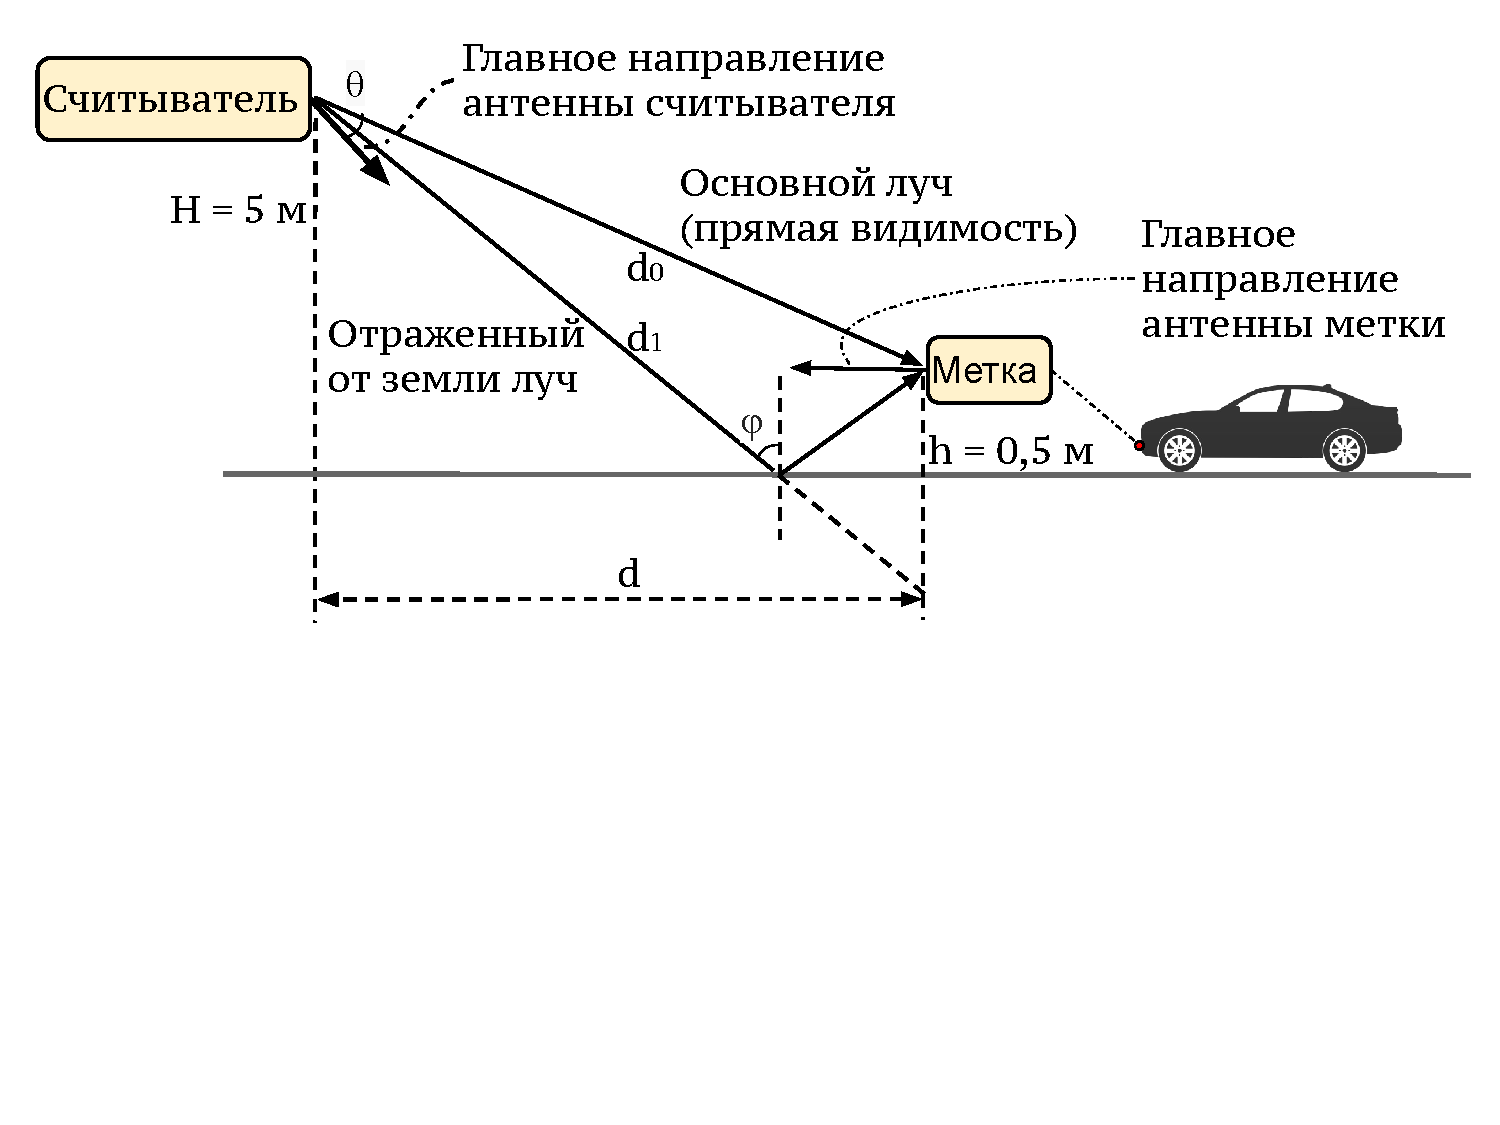
\includegraphics[width=\linewidth]{chapter2/ch2_geometry}
  }
	\caption{Схема системы радиочастотной идентификации автомобилей и ее геометрические параметры.}
	\label{fig:ch2_geometry}
\end{figure}



%%% --------------------------------------------
\subsection{Расчёт бюджета соединений}
%%% --------------------------------------------
Пусть $P_t^{(r)}$ "--- излучаемая мощность считывателя, $G^{(r)}$ "--- усиление антенны считывателя. Тогда эффективная изотропная излучаемая мощность (EIRP) составит $EIRP =  P_t^{(r)} G^{(r)}$. Здесь и далее надстрочный индекс используется для обозначения устройства: (r) для считывателя и (t) для метки; подстрочный индекс используется для обозначения направления передачи (прием или передача сигнала). При распространении сигнала от считывателя к метке сигнал испытывает затухание $A_{pl}^{(d)}$, зависящее от состояния радиоканала и взаимного расположения считывателя и метки друг относительно друга. Антенны устройств могут иметь различную поляризацию, что ведет к дополнительным потерям $A_{pol}$. Пусть усиление антенны метки равно $G^{(t)}$. Тогда мощность сигнала, принимаемого меткой, равна:

$$
	P_r^{(t)} = P_t^{(r)} G^{(r)} A_{pl}^{(d)} A_{pol} G^{(t)}.
$$

Если эта мощность меньше чувствительности метки $P_s^{(t)}$, то метка не включится и не сможет взаимодействовать со считывателем. В противном случае метка сможет передавать свои ответы за счет модулирования отраженного сигнала, мощность которого будет равна $P_t^{(t)}$. Поскольку при этом возникают дополнительные энергетические потери (например, из-за модуляции), равные $A_{bs}$, то мощность принятого и отраженного сигналов связаны как $P_t^{(t)} = P_r^{(t)} + A_{bs}$.

Для мощности сигнала, принятого от метки считывателем, можно написать следующее соотношение:

$$
	P_r^{(r)} = P_r^{(t)} G^{(t)} A_{bs} A_{pl}^{(r)} A_{pol} G^{(r)}.
$$

В общем случае потери на прямом (от считывателя к метке) и обратном (от метки к считывателю) путях могут отличаться. Это происходит из-за различия в поляризации (обычно на считывателях используются антенны с круговой поляризацией, а на метках "--- с линейной) и, как следствие, в коэффициенте отражения от земли.

\begin{table}[!t]
	\renewcommand{\arraystretch}{1.3}
	\caption{Параметры, использованные при расчете бюджета соединения}
	\label{table:ch2_budget_params}
	\centering
	\begin{tabular}{|c|c|}
		\hline
		Мощность, излучаемая считывателем, $P_t^{(r)}$ & 31.5~дБм\\
		\hline
		Усиление антенны считывателя, $G^{(r)}$ & 8~дБи\\
		\hline
		Усиление антенны метки, $G^{(t)}$ & 2~дБи\\
		\hline
		Чувствительность метки, $P_s^{(t)}$ & -18~дБм\\
		\hline
		Потери на поляризации, $A_{pol}$ & -3~дБ\\
		\hline
		Потери на модуляции на метке, $A_{bs}$ & -10~дБ\\
		\hline
		Потери в кабеле, $A_{bs}$ & -2~дБ\\
		\hline
	\end{tabular}
\end{table}

В дальнейших расчетах бюджета соединения будут использованы значения, приведенные в таблице~\ref{table:ch2_budget_params}, типичные для оборудования, применяемого в идентификации автомобилей. При расчете также следует учитывать потери в кабеле, соединяющем антенну со считывателем. Далее считается, что антенны считывателя имеют круговую поляризацию, а меток "--- линейную, таким образом потери на поляризации составляют -3~дБ.

\begin{figure}[h]
	\centerfloat{
    	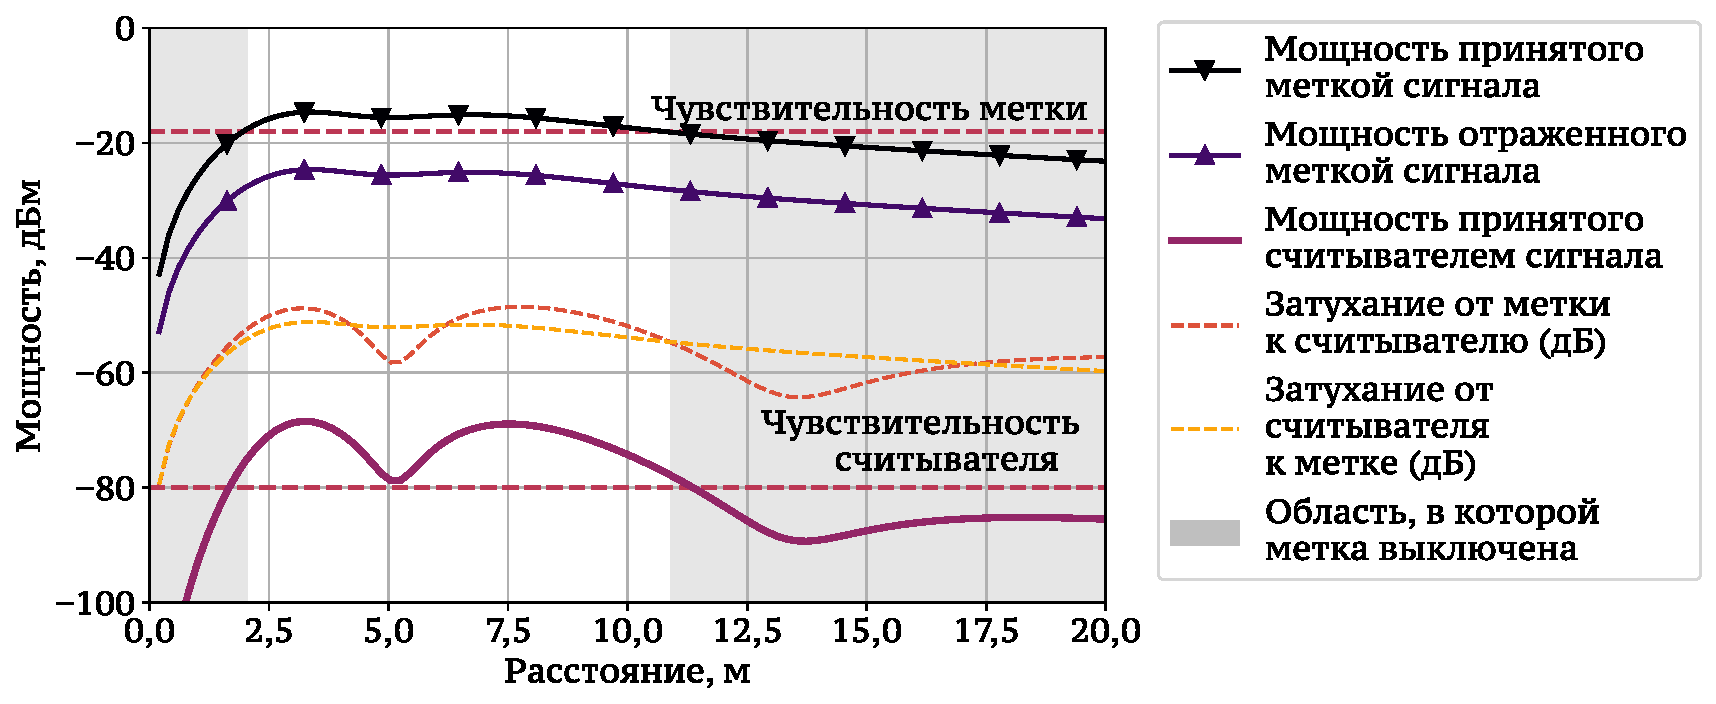
\includegraphics[width=1.0\textwidth]{chapter2/ch2_link_budget}
  	}
	\caption{Расчет бюджета соединения в зависимости от расстояния между считывателем и меткой.}
	\label{fig:ch2_link_budget}
\end{figure}

На рис.~\ref{fig:ch2_link_budget} показан расчет мощностей сигналов, принятых и переданных меткой, принятого считывателем сигнала, а также величина затухания. Все кривые убывают немонотонно из-за изменений с расстоянием в коэффициентах отражения от земли, а также из-за влияния диаграмм направленности антенн. Особенно сильно диаграмма направленности влияет на сигнал при близком расположении метки и считывателя, так как даже небольшое изменение расстояния ведет к ощутимому изменению угла падения. Для того, чтобы связь между расстоянием от считывателя до метки и временем при постоянной скорости оставалась линейной, в качестве расстояния рассматривается дистанция от опоры, на которой размещен считыватель, до метки, измеренная вдоль дороги (см. величину $d$ на рис.~\ref{fig:ch2_geometry}).



%%% --------------------------------------------
\subsection{Расчёт мощности принятых сигналов}
%%% --------------------------------------------

При движении меток и считывателей с ненулевой скоростью друг относительно друга сигналы оказываются подверженными эффекту Доплера, проявляющемуся в сдвиге частоты сигнала на величину, называемую доплеровским сдвигом, и равную:

$$
	\alpha = 1 - \frac{\upsilon \cos{\psi}}{c+\upsilon \cos{\psi}},
$$
где $c$ "--- скорость света, $\upsilon$ "--- скорость приёмника относительно передатчика, в роли приёмника может выступать как метка, так и считыватель (при этом их скорости будут иметь одинаковую величину и противоположные знаки), $\psi$ "--- угол между волновым вектором $\bm{k}$ и направлением движения, $f_c$ "--- несущая частота.

Для узкополосного сигнала в RFID-канале смещённую частоту можно приблизить выражением $\alpha f \approx f - \frac{\upsilon}{c}\cos{\psi} \cdot f_c = f - \nu$, где $\nu$ "--- доплеровский сдвиг:

$$
	\nu = \frac{\upsilon}{c} f_c\cos{\psi} = \frac{1}{2\pi}(\bm{\upsilon},\bm{k})
$$

При распространении сигнала он может отражаться от дороги, инженерных конструкций, других автомобилей и прочих объектов, то есть в моделируемой системе имеет место многолучевое распространение сигнала. При этом возникает множество копий сигнала $s(t)$, каждая из которых испытывает собственное затухание $h_i$, задержку $\tau_i$ и доплеровский сдвиг $\nu_i$, поскольку каждая копия распространяется по собственному пути, с которым, помимо длины, связаны углы передачи и приема сигнала. Пусть в сигнале присутствует прямая компонента (Line-of-Sight, LoS) сигнала и $N$ отраженных компонент (или лучей). Без потери общности рассуждений будем считать, что LoS-компонента описывается нулевым лучём, а отраженные компоненты "--- лучами $1 \dots N$. Принятый сигнал определяется следующей формулой:

\begin{equation}
	r(t) = \sum\limits_{i=0}^{N} h_i s(t-\tau_i) e^{j\nu_i t},
	\label{eq:ch2_rx_signal}
\end{equation}

Затухание $h_i$ может быть рассчитано как $h_i=\lambda/(4\pi d_i)R_i\Gamma_i$, где $\lambda$ "--- длина волны, $d_i$ "--- длина пути для $i$--го луча, $R_i$ "--- коэффициент затухания, вызванного отражением сигнала, для $i$--го луча (для основной, LoS-компоненты полагаем равным единице: $R_0=1$), $\Gamma_i = \Gamma_i^{(r)}\Gamma_i^{(t)}$ "--- ослабление сигнала, определяемое диаграммами направленности передающей и принимающей антенн.

Рассмотрим в качестве передаваемого сигнала постоянную волну (синусоидальный сигнал) единичной мощности. После подстановки формул, описанных выше, в выражение для $r(t)$ \eqref{eq:ch2_rx_signal}, получим затухание при распространении сигнала как значение мгновенной мощности на приемнике:

\begin{equation}
	A_{pl} = |r(t)|^2 = \left(\frac{\lambda}{4\pi}\right)^2
		\left|\sum\limits_{i=0}^{N} \frac{R_i\Gamma_i}{d_i}
		e^{-jk(d_i-\upsilon t \cos{\psi_i})}\right|^2
	\label{eq:ch2_pathloss}
\end{equation}

Расчёт $R_i$, $\Gamma_i$, $d_i$ и $\psi_i$ требует определения путей распространения сигнала по разным лучам. Для статического окружения, при пренебрежении отражениями от движущихся автомобилей, пути могут быть вычислены простыми аналитическими методами. При более сложном динамическом окружении (а также при моделировании отражающих объектов сложной формы) потребуется использовать техники трассировки лучей. Далее, для упрощения расчетов, будем учитывать только две компоненты: прямую (LoS) и отраженную от земли (NLoS) компоненты. Для отраженной NLoS-компоненты коэффициент затухания $R_1$ равен коэффициенту отражения от земли. Далее предполагаем, что антенна считывателя размещена на высоте 5~м, а метки "--- 0,5~м над дорогой. Остальные лучи моделируются нявно, как случайные компоненты,  обуславливающие использование распределение Рэлея при вычислении BER (подробнее об этом "--- в следующем подразделе).

\begin{figure}[h]
	\centerfloat{
    	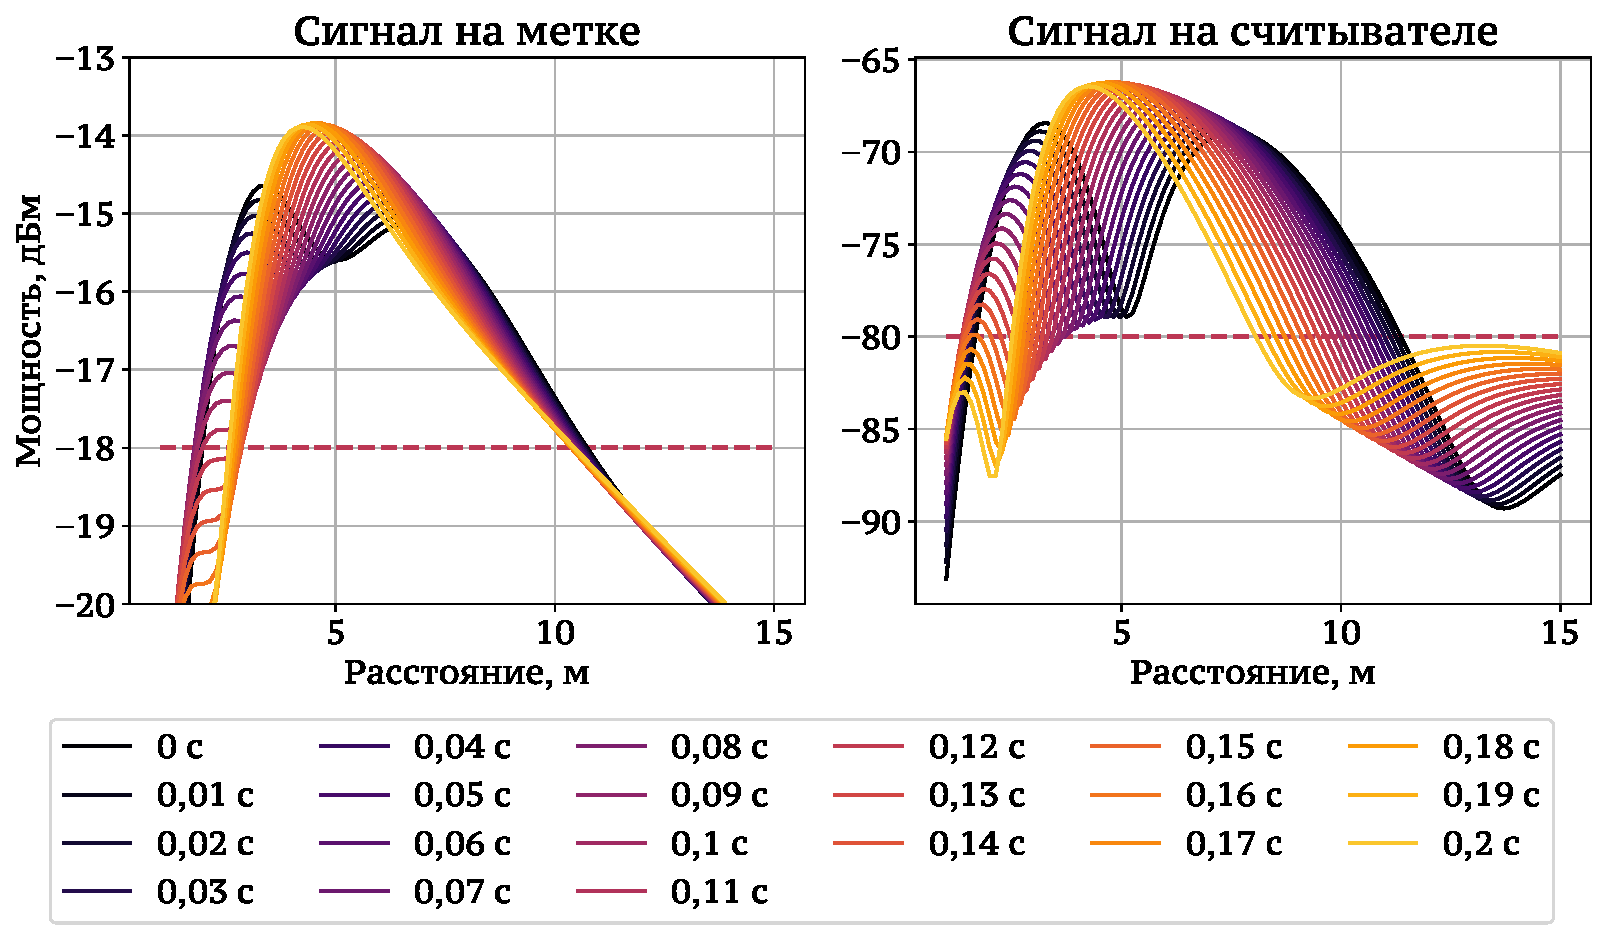
\includegraphics[width=0.95\textwidth]{chapter2/ch2_rx_power_doppler}
	}
	\caption[Зависимость мощности сигналов, принятых меток и считывателем, от расстояния и времени]{Зависимость мощности сигнала, принятого считыватлем, от расстояния между считывателем и меткой $d$ и временем, прошедшим с начала приема меткой сигнала от считывателя}
	\label{fig:ch2_rx_power_doppler}
\end{figure}

Наличие эффекта Доплера делает канал зависимым от времени (см. \cite{Matz2011}), поскольку, как видно из формулы \eqref{eq:ch2_rx_signal}, величина сдвига для каждого луча определяется индивидуально и зависит от времени, прошедшего с начала получения сигнала. Особенность RFID-системы состоит в том, что считыватель не перестает передавать сигнал (постоянный, который метка может модулировать для передачи своего ответа, или информационный) ни после передачи своей команды, ни после получения ответа. Считыватель может прекращать передачу сигнала, например, для сброса флагов сессий меток, при переключении частот или в том случае, если по законодательству он должен периодически освобождать радиоканал. Однако, такие прерывания происходят относительно редко, внутри одного или нескольких раундов сигнал не прерывается. Поэтому значение $t$ в \eqref{eq:ch2_rx_signal} определяется как время, прошедшее со включения считывателя, за вычетом длительности распространения сигнала от считывателя до метки. Хотя метка в это время может еще находиться далеко, радиоканал уже будет существовать. Учитывая, что в момент включения считывателя метки расположены на разных расстояниях от считывателя, получаем, что значение $t$ в одной и той же точке для разных меток будет разным, а соответственно разными будут и значения $r(t)$. На рис.~\ref{fig:ch2_rx_power_doppler} показана зависимость мощностей сигналов, принятых меткой и считывателем, от расстояния $d$, измеренного вдоль дороги. Различные кривые соответствуют времени, прошедшему с начала приема меткой сигнала от считывателя.

\begin{figure}[h]
	\centerfloat{
    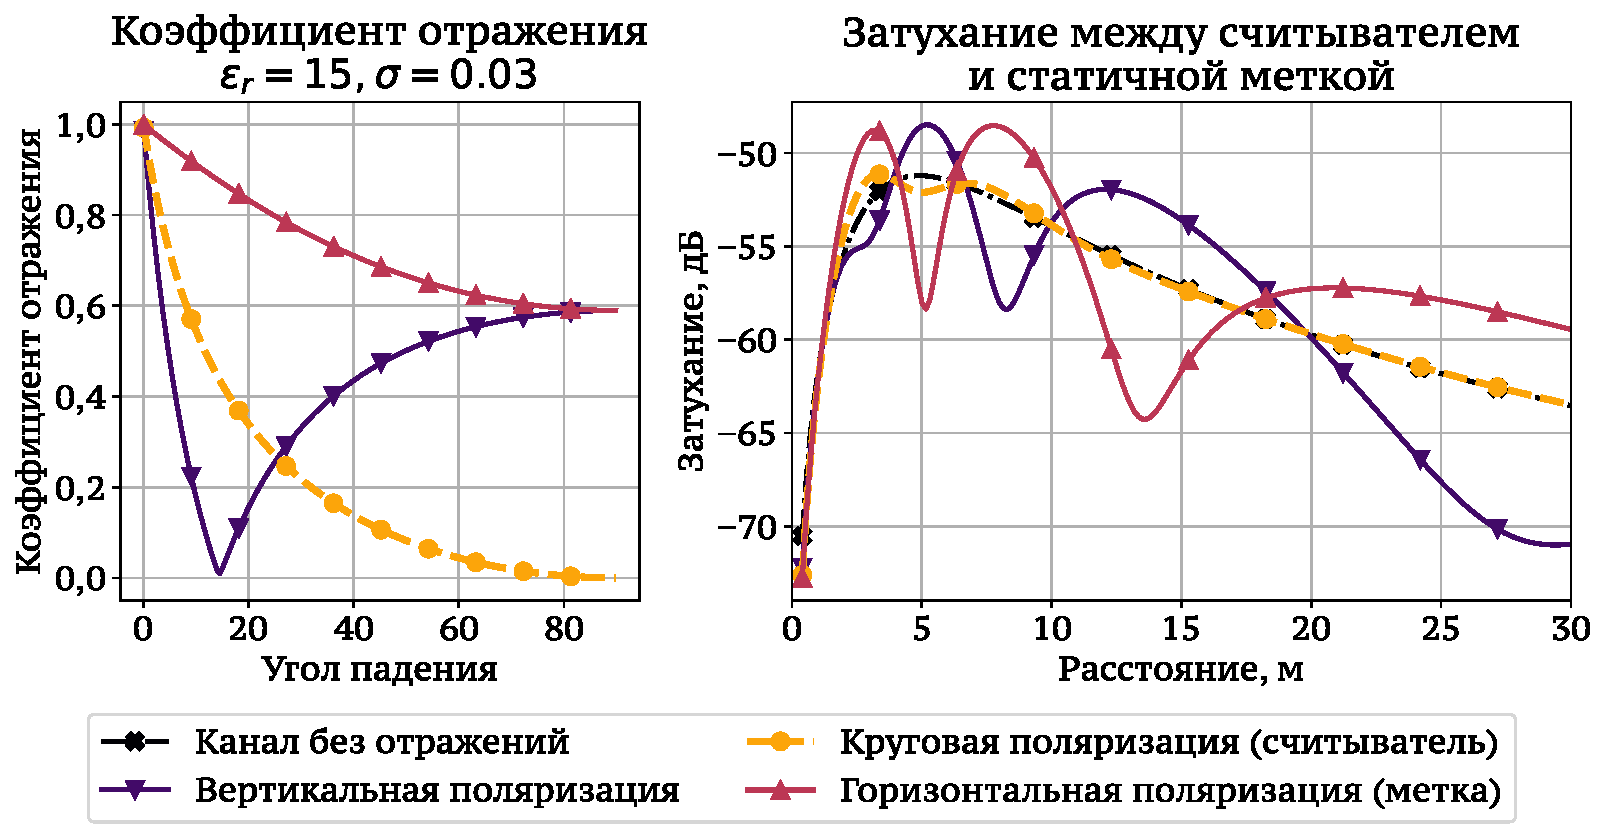
\includegraphics[width=0.9\textwidth]{chapter2/ch2_pathloss}
  }
	\caption{Коэффициент отражения и затухание сигнала для параллельной, перпендикулярной и круговой поляризаций}
	\label{fig:ch2_pathloss}
\end{figure}

На рис.~\ref{fig:ch2_pathloss} показаны результаты расчета затухания сигнала в зависимости от расстояния для разных видов поляризации: параллельной, перпендикулярной и круговой. Различие обусловлено тем, что коэффициент отражения от земли $R_1$ для NLoS-компоненты сигнала принимает разные значения в зависимости от выбранной поляризации. Коэффициент отражения определен следующей формулой \cite{Gonzalez2013}:
$$
  R = \frac{\sin\phi - \sqrt{C}}{\sin\phi + \sqrt{C}},
$$
где $\phi$ "--- угол падения, $C = \eta - \cos^2\phi$ для горизонтально поляризованной компоненты и $C = \frac{\eta - \cos^2\phi}{\eta^2}$ для вертикально поляризованной; $\eta = \epsilon_r(f)-j60\lambda\sigma(f)$, где $\epsilon_r(f)$ "--- относительная диэлектрическая проницаемость поверхности для заданной частоты $f$, $\sigma(f)$ "--- проводимость.

\begin{figure}[h]
	\centerfloat{
    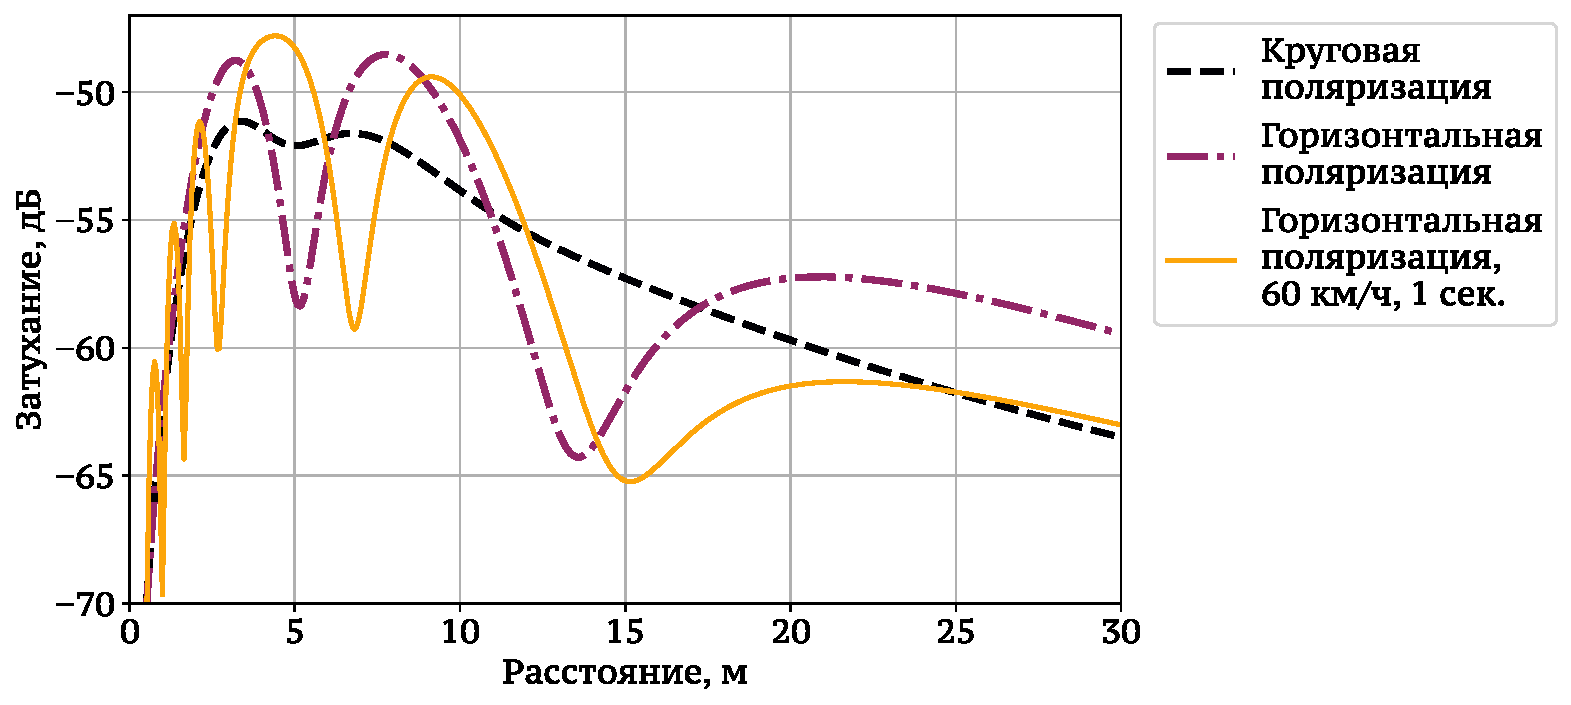
\includegraphics[width=0.9\textwidth]{chapter2/ch2_pathloss_3}
  }
	\caption{Зависимость коэффициента отражения от угла падения для параллельной, перпендикулярной и круговой поляризации при разных значениях относительной диэлектрической проницаемости $\epsilon$ и проводимости $\sigma$.}
	\label{fig:ch2_pathloss_3}
\end{figure}

Относительная диэлектрическая проницаемость и проводимость сильно зависят от влажности поверхности. Проводимость $\sigma$ меняется в диапазоне от 0.00014~См/м для очень сухой земли до 5~См/м для морской воды. Относительная диэлектрическая проницаемость $\epsilon_r$ меняется в диапазоне от 3 до 70. В дальнейшем будем использовать значения проводимости $\sigma = 0,03$~См/м и диэлектрической проницаемости $\epsilon_r = 15$, характерные для сухой дороги с твердым покрытием.

Одновременный учет коэффициента отражения и эффекта Доплера делают зависимость затухания от расстояния достаточно сложной. На рис.~\ref{fig:ch2_pathloss_3} показан пример расчета величины затухания для круговой и горизотнальной поляризаций в момент времени $t = 0$ и через 1 секунду после включения считывателя.

Наконец, для расчета мощностей сигналов необходимо учитывать диаграммы направленности антенн. Будем считать, что у метки простая дипольная антенна, и её диаграмма направленности определяется как:

\begin{equation}\label{eq:ch2_dipole}
	\Gamma(\theta) = \left|
		\frac{\cos{\frac{\pi}{2}\sin{\theta}}}{\cos{\theta}} \right|,
\end{equation}

Для простоты, будем считать, что диаграмма антенны считывателя также определяется с помощью~\eqref{eq:ch2_dipole}. Для более точного расчета можно использовать более подходящие диаграммы, например "--- патч-антенны \cite{Balanis2016}.




%%% --------------------------------------------
\subsection{Расчёт вероятности битовой ошибки (BER)}
%%% --------------------------------------------
\begin{figure}[h]
	\centerfloat{
    	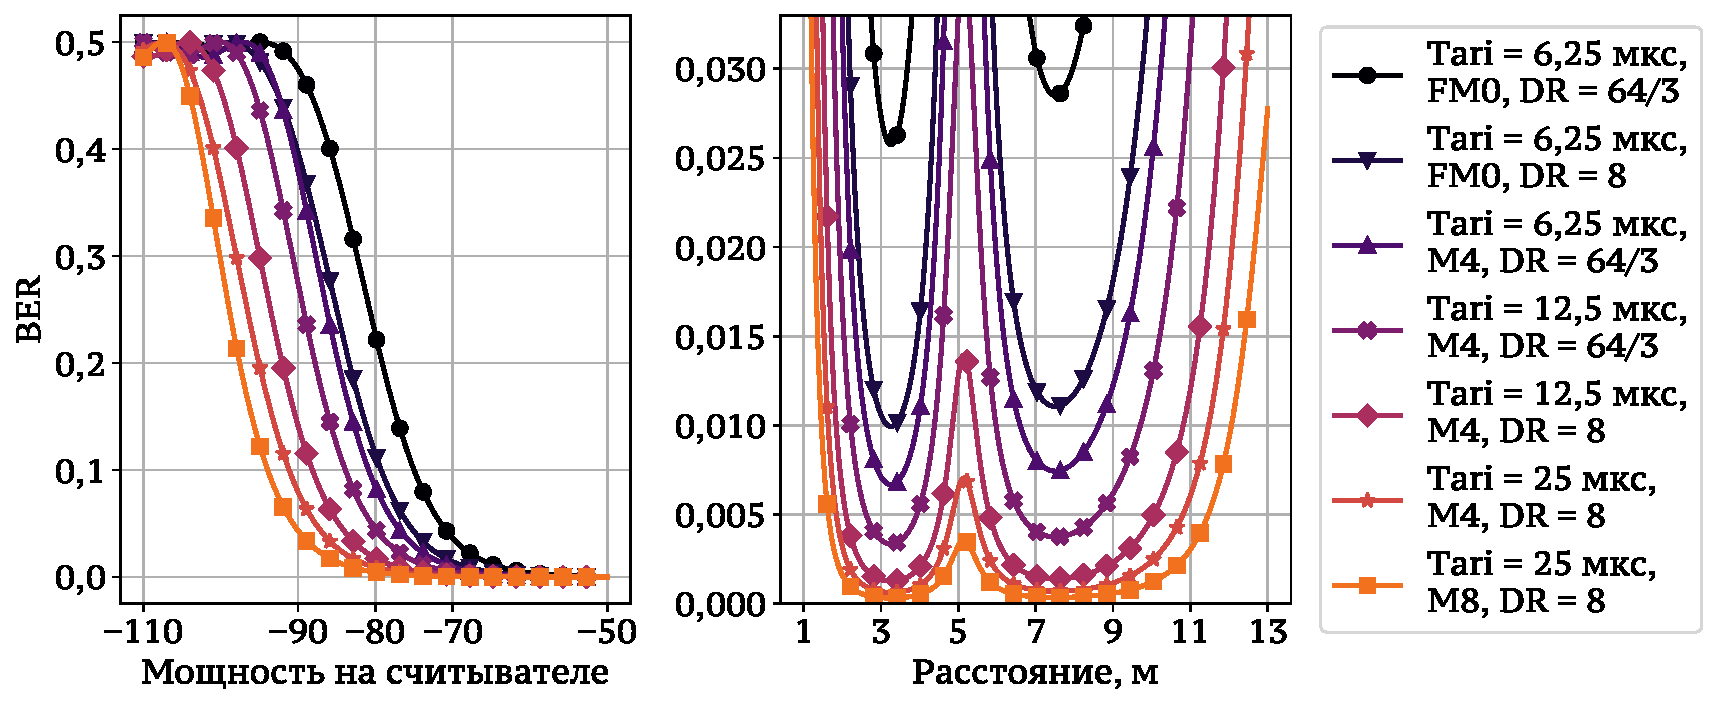
\includegraphics[width=1.0\textwidth]{chapter2/ch2_ber}
  	}
	\caption{Вероятность битовой ошибки (BER) для разных параметров Tari и M.}
	\label{fig:ch2_ber}
\end{figure}

Рассмотрим радиоканал с аддитивным гауссовским шумом (AWGN). Вероятность ошибки в передаче бита (BER) можно выразить следующей формулой:

\begin{equation}
	P_{er} = 2Q(\acute{\gamma})[1-Q(\acute{\gamma})],
	\label{eq:ch2_awgn}
\end{equation}
где $Q(\cdot)$ "--- Q--функция; $\acute{\gamma} = mE_s/N_0\cos^2{\phi_s}$; $m$ "--- число символов на бит (порядок) в коде Миллера, $E_s$ "--- энергия одного символа, $N_0/2$ "--- спектральная плотность белого шума и $\phi_s$ "--- разность между реальной и принятой фазами сигнала. Соотношение $E_s/N_0$ может быть выражено как $\gamma T_s B$, где $\gamma$ отношение сигнал-шум (SNR), $T_s$ "--- длительность символа и $B$ "--- ширина полосы. Ошибку синхронизации фазы будем приближенно моделировать как $\cos^2{\phi_s} \approx 1/\gamma T_{pr}B$, где $T_{pr}$ "--- длительность преамбулы \cite{RFID_JRFID2017}.

Использование гауссовской модели оказывается слишком оптимистичным, так как при расчете мощности принятого сигнала учитываются не все лучи. Далее будет использоваться выражением, получаемым усреднением $P_{er}$ в формуле \eqref{eq:ch2_awgn} по $\acute{\gamma}$, которую считаем случайной величиной, имеющей распределение Рэлея \cite{Lazaro2009}:

$$
	P_{er} = \frac{1}{2} - \frac{1}{\sqrt{1+\frac{2}{\acute{\gamma}}}} +
			 \frac{2}{\pi}\frac{\arctan{\sqrt{1+\frac{2}{\acute{\gamma}}}}}{1+\frac{2}{\acute{\gamma}}}.
$$

\begin{figure}[h]
	\centerfloat{
    	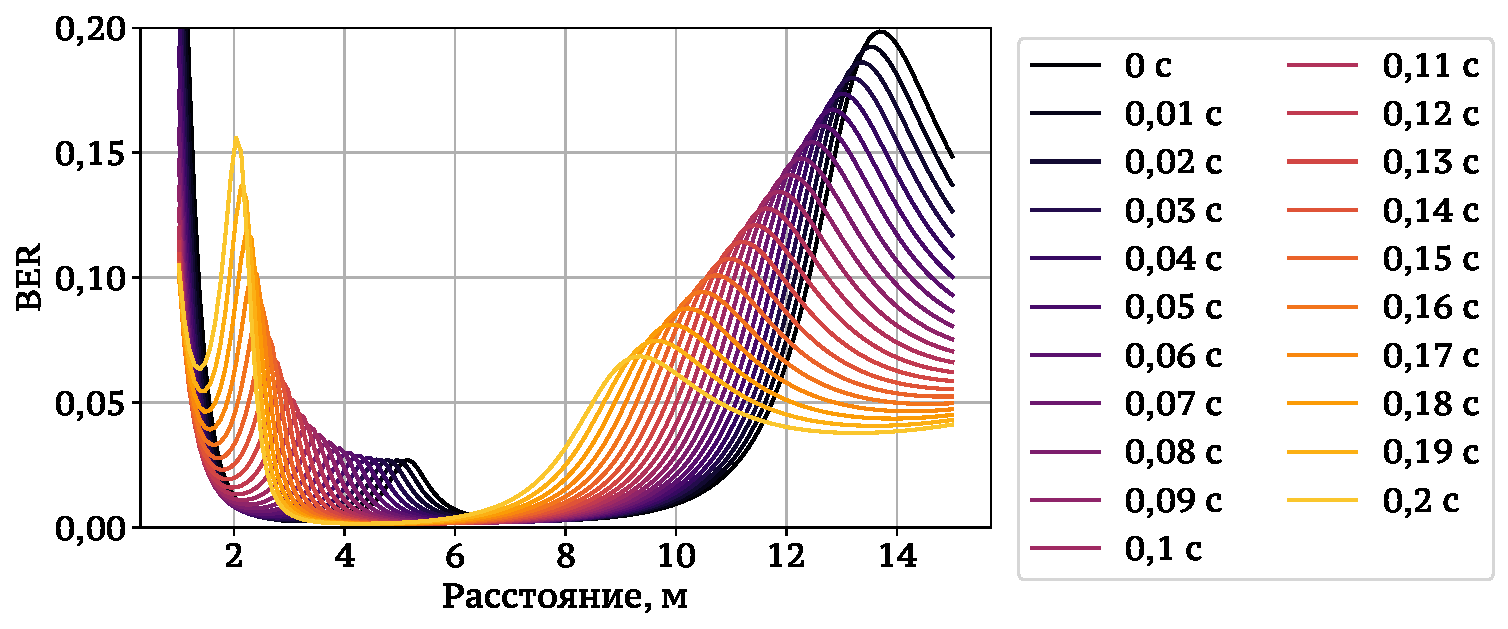
\includegraphics[width=1.0\textwidth]{chapter2/ch2_ber_doppler}
  	}
	\caption{Изменение вероятности битовой ошибки (BER) из-за эффекта Доплера.}
	\label{fig:ch2_ber_doppler}
\end{figure}

На рис.~\ref{fig:ch2_ber} показана зависимость BER от выбранного типа кодирования ответа метки. Как и следовало ожидать, при росте числа символов на бит $m$ и уменьшении BLF (при увеличении Tari и уменьшении DR) BER снижается. Так, при Tari = 6,25~мкс, коде FM0 (m = 1) и DR = 64/3 BER не опускается ниже 0,025, в то время как при Tari = 25 мкс, коде Miller-8 (m = 8) и DR = 8 BER оказывается ниже 0,001 в области размером около 5 метров. При этом число попыток передать свой идентификатор у метки, то есть число раундов, зависит от тех же параметров противоположным образом (см. рис.~\ref{fig:ch2_max_num_rounds}).

Для успешной передачи EPCID метке нужно передать без ошибок RN16 (16 бит) и ответ на ACK, содержащий EPCID, PC (16 бит) и CRC (16 бит). Полагая длину EPCID, равной 96 битам, в общей сложности метка должна передать 144 бита. При BER = 0,01 вероятность успешной передачи составит 23,5\%, при BER = 0,005 "--- 48,8\%, а при BER = 0,001 "--- 86,5\%. Учитывая, что метка может принять участие только в небольшом количестве раундов (см. рис.~\ref{fig:ch2_max_num_rounds}), нужно выбирать такие параметры протокола, при которых область с низким BER будет достаточно большой, и при этом метка должна успеть совершить несколько попыток передачи идентификатора. Отметим, что из-за немонотонной зависимости BER от расстояния, такая область разбивается на <<окна>>, а из-за эффекта Доплера (см. рис.~\ref{fig:ch2_ber_doppler}) эти <<окна>> смещаются с течением времени от включения считывателя.



%%%%%%%%%%%%%%%%%%%%%%%%%%%%%%%%%%%%%%%%%%%%%%%%%%%%%%%%%%%%%%%%%%%%%%%%%%%%%%%%
\section{Результаты имитационного моделирования}\label{sec:ch2_results}
%%%%%%%%%%%%%%%%%%%%%%%%%%%%%%%%%%%%%%%%%%%%%%%%%%%%%%%%%%%%%%%%%%%%%%%%%%%%%%%%
Для проведения численного эксперимента была разработана имитационная модель на языке Python. Исходный код модели, документация и собранные данные можно найти в Git-репозитории на GitHub: \url{https://github.com/larioandr/thesis-rfidsim}.

Разработанная дискретно-событийная имитационная модель "--- достаточно гибкая и простая, позволяет легко вносить изменения для адаптации к другим экспериментам. Состояние модели изменяется при наступлении различных событий "--- начала и окончания приема сигнала, окончания ожидания сообщения, обновления положения меток, таймаута для переключения антенны считывателя, генерации нового автомобиля с меткой и прочих. Для того, чтобы учесть изменение мощностей сигналов при движении метки, затухания и мощности пересчитывались периодически при обновлении положения метки (каждую миллисекунду модельного времени), и записывались для дальнейшего определения минимального уровня сигнала и расчета BER. Более подробное описание модели можно найти в репозитории. Главный недостаток модели "--- высокая вычислительная сложность. Так, для получения численных результатов, представленных в диссертационном исследовании, потребовалось около восьми часов выполнения модели на четырехядерном сервере Модель имеет более 50 параметров, в том числе:
\begin{itemize}
	\item настройки протокола: интервалы Tari, RTcal, TRcal, метод кодирования ответов меток (M), коэффициент DR, использовать ли расширенную преамбулу (TRext);
	\item параметры мобильности меток: скорость движения, частота генерации;
	\item параметры окружения: число и ширина полос движения, длина автомобилей, относительная диэлектрическая проницаемость и проводимость дорожного покрытия, уровень шума;
	\item параметры считывателя: мощность передатчика, потери в кабеле, поляризация, усиление, диаграмма, высота и угол наклона антенн, порядок выбора флагов сессии для опроса;
	\item параметры меток: высота установки, поляризация, усиление и диаграмма антенн, потери на отражении сигнала, длина EPCID и TID, чувствительность;
	\item параметры канала: учиытвать ли эффект Доплера, модель для расчета BER.
\end{itemize}

В ходе численного эксперимента были получены оценки идентификации автомобилей, на которых были установлены RFID-метки. Автомобиль считался идентифицированным, если была успешно прочитана хотя бы одна метка в переднем или заднем номере. Кроме того, для более глубокого понимания работы системы, было исследовано число раундов, в которых успевает принять участие движущаяся метка.



%%% --------------------------------------------
\subsection{Анализ влияния частоты переключений антенн на число раундов}
%%% --------------------------------------------
Точное число раундов, в которых успевает принять участие метка, зависит как от настроек протокола (схема кодирования ответов метки, выбор параметра Q и пр.), так и от алгоритма выбора сессии и частоты смены антенн. Так как вероятность прочитать и EPCID, и TID в одном раунде относительно мала, существенным оказывается то, в скольких раундах метка успевает принять участие, т.е. сколько у нее будет попыток передать свои идентификаторы.

В начале раунда инвентаризации считыватель выбирает сессию (S0, S1, S2, S3) и значение её флага ($A$ или $B$). Метка отвечает только в том случае, если хранимеый ею флаг выбранной сессии совпадает с переданным в команде Query. После рассылки своего EPCID в ответе на ACK, метка инвертирует значение хранимого флага сессии ($A \rightarrow B,\, B \rightarrow A$). Для каждой сессии стандарт определяет интервал времени после выключения питания, в течение котрого метка должна сохранять значение флага сессии, а после которого, если питания так и не появилось, "--- возвращать значение $A$. В дальнейшем будем рассматривать сессию S0, для которой эта процедура самая прстая "--- значение $A$ должно быть установлено сразу после сброса питания, независимо от длительности потери энергии.

\begin{figure}[h]
	\centerfloat{
    	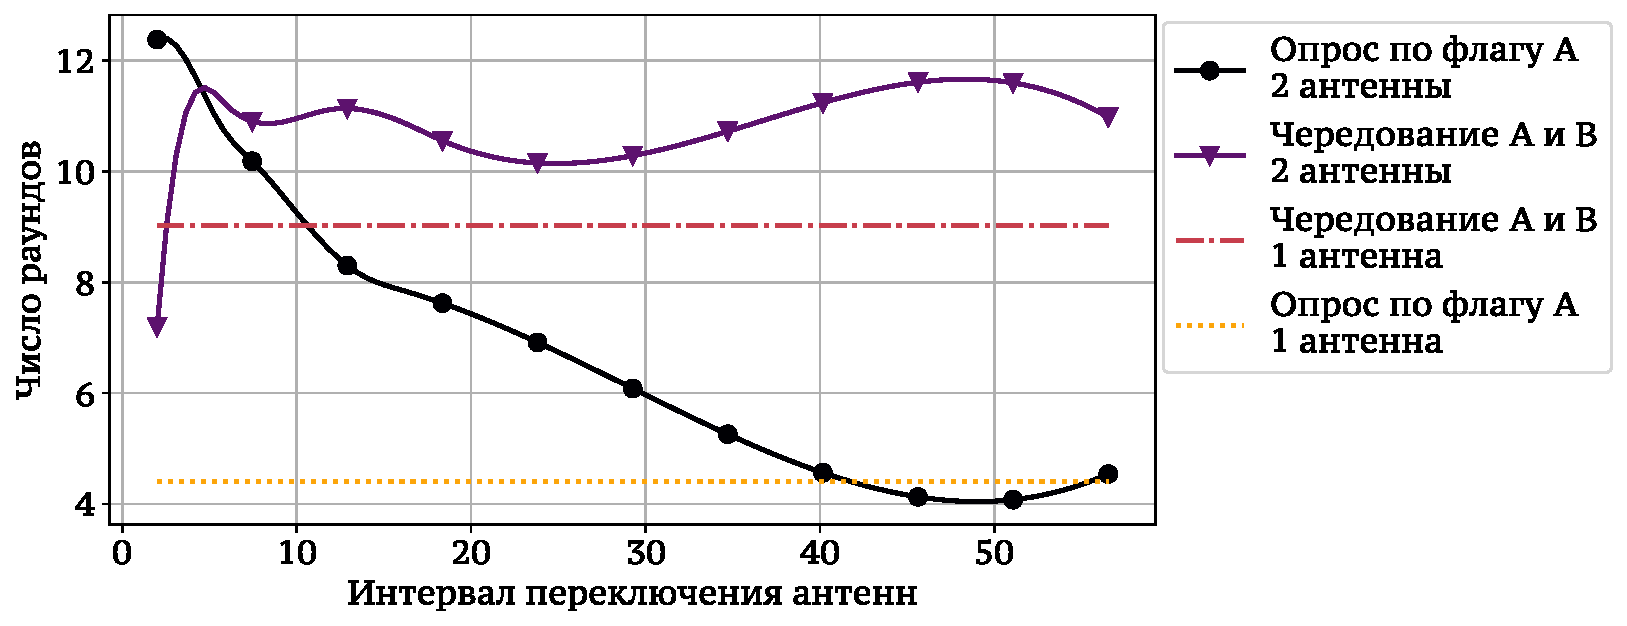
\includegraphics[width=1.0\textwidth]{chapter2/ch2_sim_num_rounds_one_lane}
  	}
	\caption{Число раундов, в которых участвует метка, в зависимости от длительности работы на одной антенне, для разных стратегий выбора флага сессии.}
	\label{fig:ch2_rounds_per_tag}
\end{figure}

Если считыватель использует одну антенну без периодического выключения питания, число раундов, в которых участвует метка, зависит только от стратегии выбора флага сессии. На рис.~\ref{fig:ch2_rounds_per_tag} приведены результаты симуляции, которые показывают, что число раундов при опросе меток только со значением флага сессии S0 = $A$ (самая нижняя горизонтальная линия) и число раундов при смене значений запрашиваемых флагов каждый раунд отличаются в шесть раз. В первом случае число раундов, в которых принимает участие метка, определяется только числом включений метки (выключения обусловлены приемом сигнала считывателя на уровне, меньшем чувствительности метки). При периодической смене флагов метка имеет возможность повторно участвовать в опросе и без выключения, поэтому число раундов оказывается значительно больше, а тем самым повышается вероятность того, что хотя бы один раз метка успешно передаст свои идентификационные данные. Небольшие колебания на приведенном графике обусловлены случайным характером процесса чтения меток, а также случайностью длительности раундов, зависящей от числа занятых и пустых слотов. Также следует отметить, что на число раундов может влиять выбор параметра Q (график соответствует значению Q = 2), а также использование операции Select, которая в представленном исследовании не использовалась.

Если считыватель использует несколько антенн и периодически между ними переключается, число раундов также зависит от интервала между переключениями антенн. На рис.~\ref{fig:ch2_rounds_per_tag} показаны результаты, полученные исходя из того, что считыватель размещен над однополосной дорогой и оборудован двумя антеннами, направленными в противоположные стороны (для чтения переднего и заднего номеров). Можно видеть, что периодическая смена флагов сессии также позволяет увеличить число раундов, хотя и меньше, чем при использовании одной антенны. Можно заметить, что сильнее всего выбор интервала переключения антенн влияет на число раундов при малых значениях интервала. Это связано, в первую очередь, с тем, что при этом переключение происходит каждый раунд или быстрее, метка может не успеть передать свой EPCID до потери энергии (здесь предполагается, что переключение антенн не связано с границами раунда, что является некоторым упрощением). Это связано, в первую очередь, с тем, что периоды работы на одной антенне быстро становятся сопоставимыми с длительностью проезда зон с уровнем сигнала от считывателя, превышающим чувствительность меток. При увличении мощности сигнала или чувствительности меток зависимость должна оказываться более сильной.

Следует отметить, что при использовании других сессий (например, S2), результаты оказываются ближе к случаю отсутствия переключения антенн для малых интервалов, так как при малых интервалах между переключениями (меньших, чем время сохранения флага сессии) метка может <<не заметить>> потерю энергии и сохранить значение флага.

На число раундов также влияет длительность работы считывателя до его выключения и время нахождения в выключенном состоянии. Все расчёты в этом и следующем разделе сделаны в предположении, что считыватель выключается каждые 2 секунды на 100 милисекунд.



%%% --------------------------------------------
\subsection{Анализ вероятности идентификации транспортных средств}
%%% --------------------------------------------
С помощью имитационной модели была изучена вероятность идентификации меток, расположенных на номерах автомобилей, двигающихся по однополосной дороге. Считыватель был оборудован двумя антеннами, размещенными над дорогой в противоположных направлениях, для чтения переднего и заднего знаков.

Для выбора параметра Q было рассчитано среднее число меток, участвующих в одном раунде. Результаты этого расчета приведены в табл.~\ref{table:ch2_tags_num_per_round}, где $N_v$ "--- среднее число автомобилей вблизи считывателя, $T_v$ "--- средний интервал времени между появлениями автомобилей, $N_t$ "--- среднее число меток, участвующих в раунде, а $N_t^{(1)}$ "--- среднее число меток в тех раундах, в которых участвует хотя бы одна метка. Из приведенных результатов видно, что даже при очень интенсивном потоке, когда в зоне действия считывателя оказывается более пяти машин, из-за неравномерности уровня сигнала большая часть меток оказывается выключенными, и можно считать, что в каждом раунде участвует не более одной метки. Фактически это означает, что вероятностью коллизий можно пренебречь и выбирать значение Q сколь угодно малым, так как его увеличение лишь добавит пустых слотов. Учитывая, что длительность пустого слота достаточно мала и для перестраховки на тот случай, когда помимо меток в номерех в зону действия попадут  другие метки (расположенные, например, на предметах под стеклом автомобиля или на самом автомобиле), можно установить Q=2. В дальнейшем это значение будет использовано для получения остальных результатов.

\begin{table}[h]
	\renewcommand{\arraystretch}{1.3}
	\caption{Среднее число меток, участвующих в раунде, при движении автомобилей со скоростью 60~км/ч}
	\label{table:ch2_tags_num_per_round}
	\centering
	\begin{tabular}{|c|c|c|c|}
		\hline
		$T_v$, sec & $N_v$ & $N_t$ & $N_t^{(1)}$ \\\hline
		0.5 & 5.67 & 0.1000 & 1.0 \\\hline
		1.0 & 3.38 & 0.0357 & 1.0 \\\hline
		\end{tabular}
\end{table}


\begin{figure}[h]
  \centerfloat{
    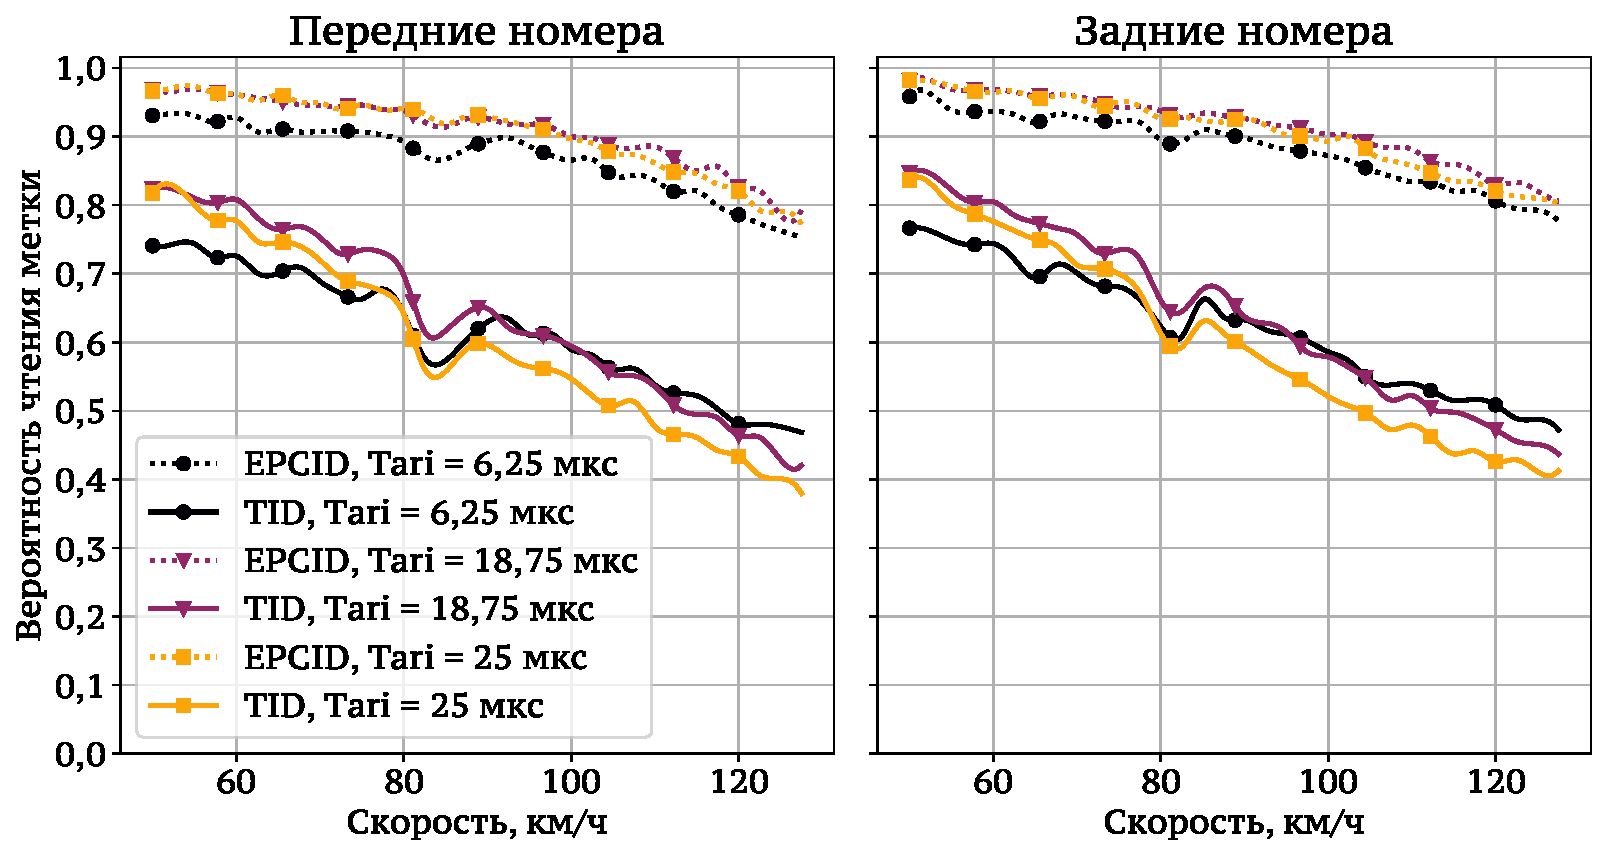
\includegraphics[width=1.0\textwidth]{chapter2/ch2_tag_identification_m4}
  }
	\caption{Вероятность успешного чтения меток в номерах при различных значениях Tari и кодировании ответов M = 4}
	\label{fig:ch2_tag_identification_m4}
\end{figure}

\begin{figure}[h]
  \centerfloat{
    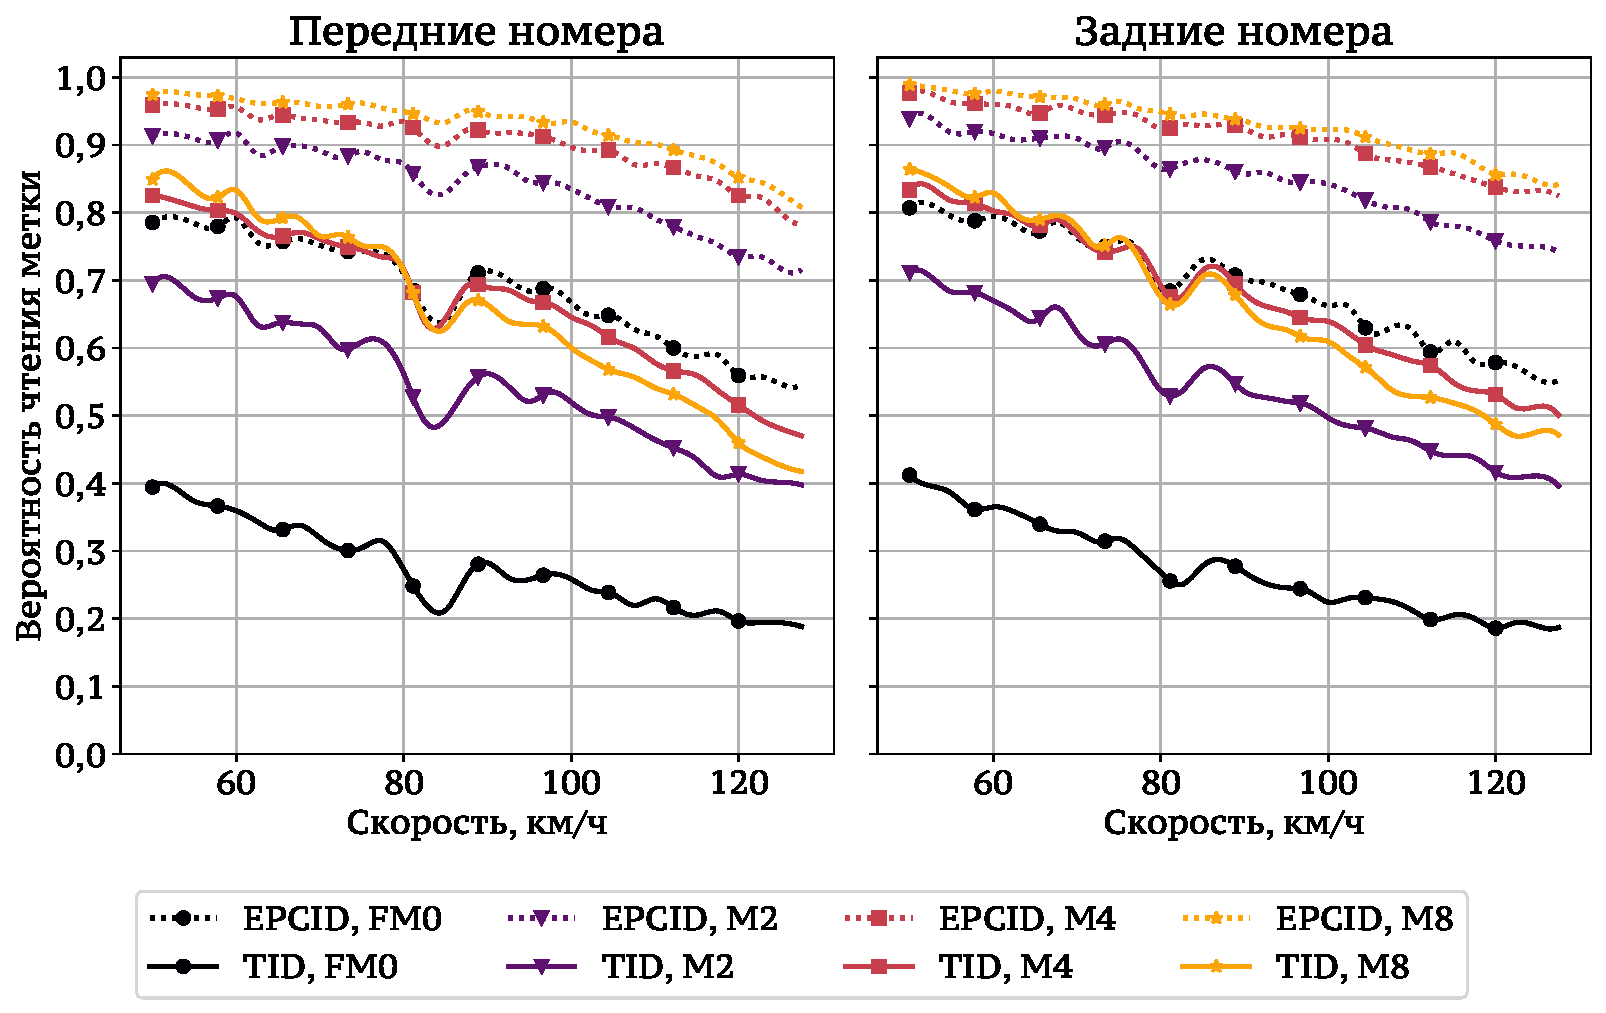
\includegraphics[width=1.0\textwidth]{chapter2/ch2_tag_identification_tari125}
  }
	\caption{Вероятность успешного чтения меток в номерах при различных значениях M и Tari = 12,5~мкс}
	\label{fig:ch2_tag_identification_tari125}
\end{figure}

На рис.~\ref{fig:ch2_tag_identification_m4} и \ref{fig:ch2_tag_identification_tari125} показаны результаты расчёта вероятности идентификации меток в номерах в заивисимости от скорости движения автомобилей при различных значениях интервала Tari (см. рис.~\ref{fig:ch2_tag_identification_m4}) и различных значениях M (число символов на бит в ответах меток, см. рис.~\ref{fig:ch2_tag_identification_tari125}). Предполагалось, что антенны считывателя имеют усиление 8~дБи, потери в кабеле составляют 2~дБ, метки используют расширенные преамбулы, а значение DR=8. Считыватель работал в сессии S0, инвертировал значение флага сессии в каждой команде Query и переключал антенны каждые 100~мс. Из приведенных графиков видно, что вероятность чтения меток падает с ростом скорости. При этом вероятность чтения EPCID остаётся высокой при достаточно больших скоростях свыше 120~км/ч, чего нельзи сказать про чтение TID. Важно отметить, что выбор больших значений Tari не обязательно ведет к увеличению вероятности успешной идентификации (см. рис.~\ref{fig:ch2_tag_identification_m4}), также как и выбор больших значений M (см. рис.~\ref{fig:ch2_tag_identification_tari125}). Более того, при чтении TID выбор самых больших значений Tari = 25~мкс и M = 8 даёт результаты хуже, чем выбор менее надёжных значений Tari = 18,75~мкс и M = 4, хотя выбор еще меньших значений также снижает вероятность успешного чтения. Объяснить эту закономерность можно тем, что выбор слишком больших значений ведёт к увеличению длительности раундов и, как следствие, снижению вероятности успешной идентификации хотя бы в одном раунде, хотя и повышает вероятность успешного чтения TID в одном раунде. Дальнейшее же уменьшение значений M и Tari ведет к слишком сильному уменьшению вероятности успешной передачи в одном раунде. Этот вывод подтверждается также тем, что выбор оказывается менее существенным при чтении только EPCID, так как и увеличение длительности раунда там оказывается менее значительным, и влияние вероятности успешной передачи ответов метки меньше зависит от BER (так как в этом случае ответов, которые должна передать метка, в два раза меньше).

\begin{figure}[h]
  \centerfloat{
    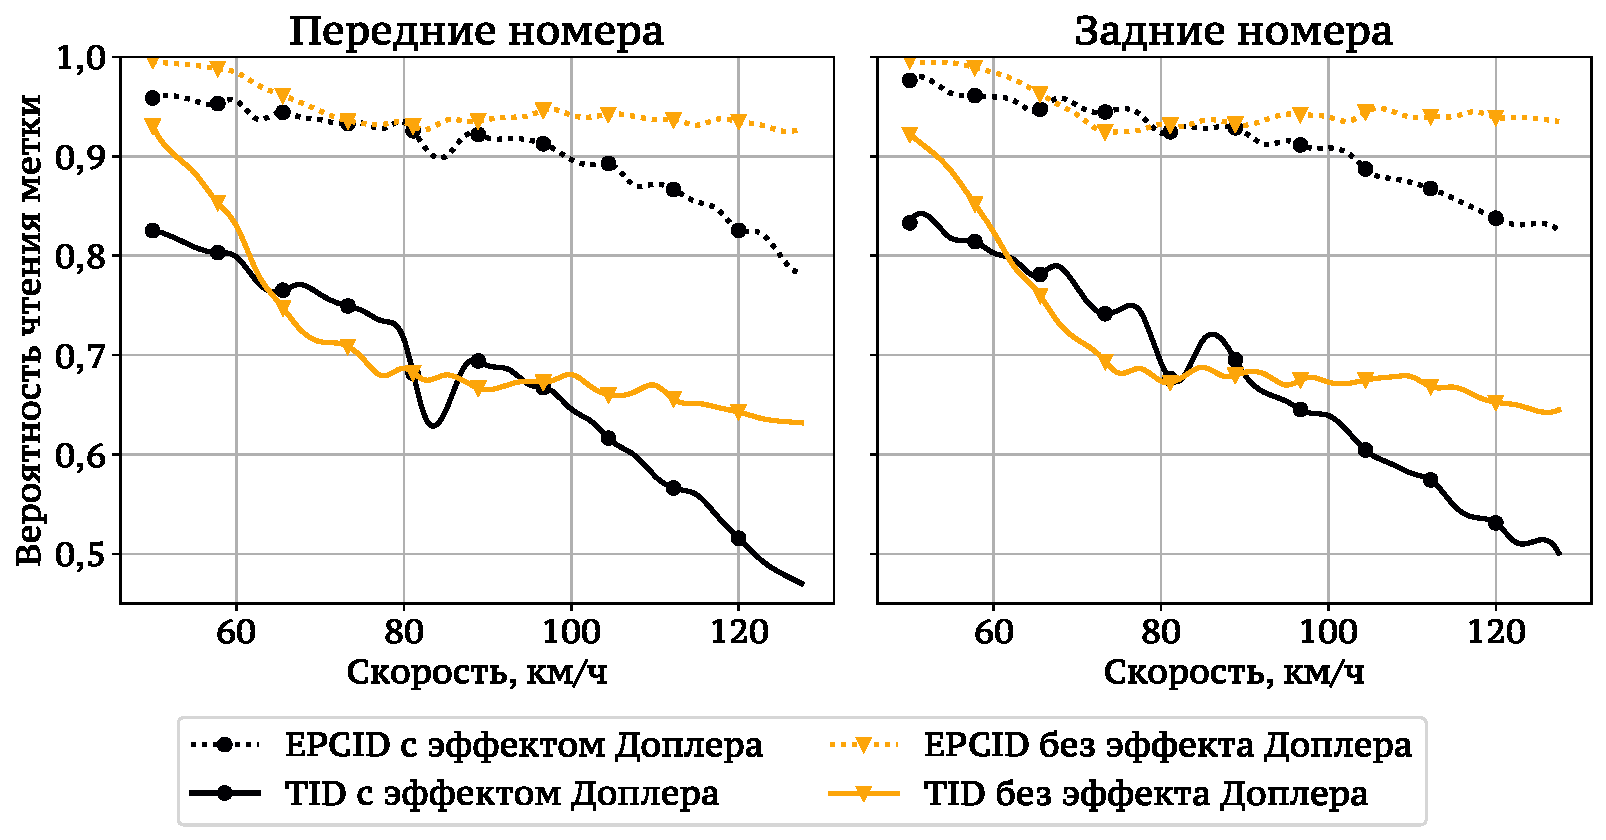
\includegraphics[width=1.0\textwidth]{chapter2/ch2_identification_doppler}
  }
	\caption{Влияние эффекта Доплера на вероятность успешного чтения метки при M = 4, Tari = 12,5~мкс}
	\label{fig:ch2_identification_doppler}
\end{figure}

Также было проведено численное исследование влияния эффекта Доплера, см. рис.~\ref{fig:ch2_identification_doppler}. Как видно из приведённых результатов, эффект Доплера оказывает существенное влияние на вероятность чтения меток, особенно при чтении TID на высоких скоростях "--- в этом случае эффект Доплера может снижать вероятность успешного чтения метки на 10--20~\%.

\begin{figure}[h]
	\centerfloat{
    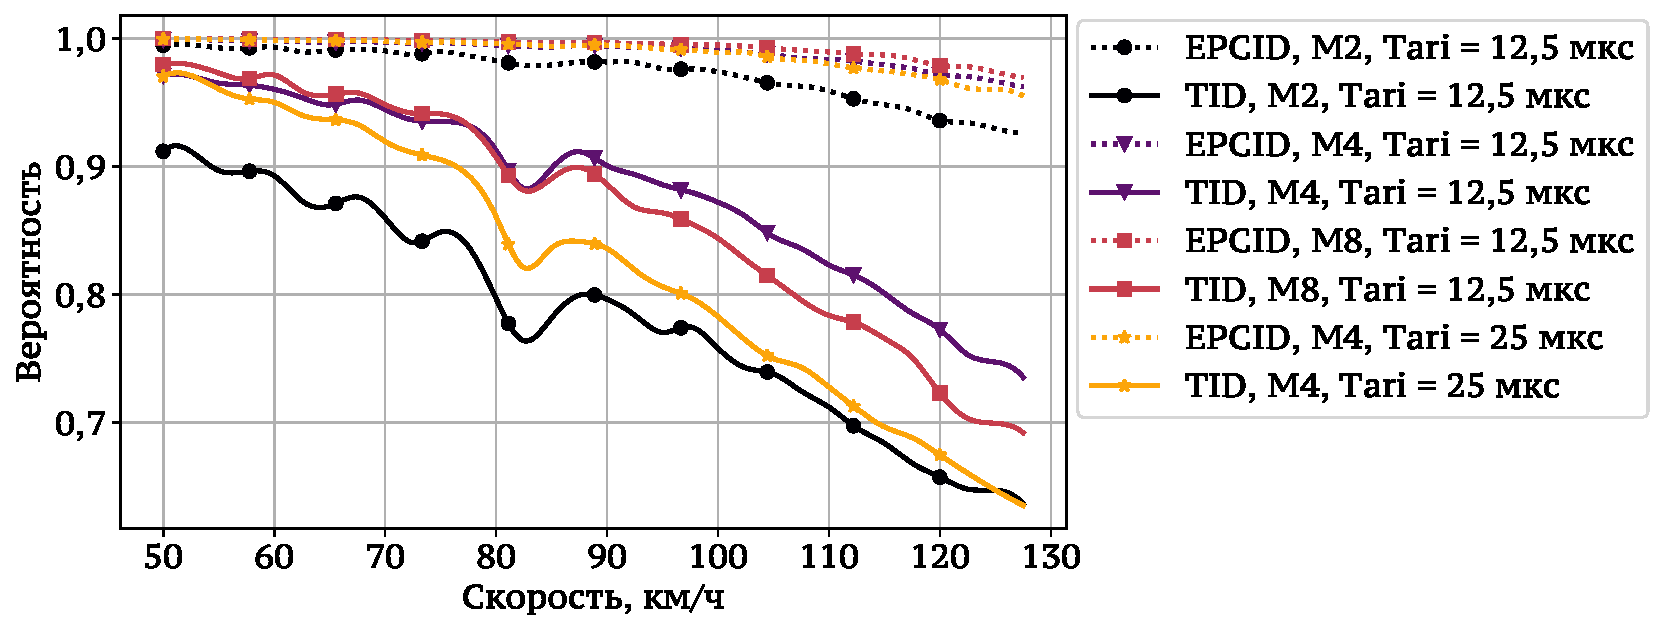
\includegraphics[width=1.0\textwidth]{chapter2/ch2_vehicle_identification_rate}
  }
	\caption{Вероятность идентификации автомобиля с метками на переднем и заднем номере, идентифицируемого по любой из меток}
	\label{fig:ch2_vehicle_identification_rate}
\end{figure}

Результаты расчета вероятности идентификации автомобилей показаны на рис.~\ref{fig:ch2_vehicle_identification_rate}. При проведении расчётов считалось, что автомобиль может быть идентифицирован по любой метке, т.е. для успешной идентификации было достаточно единожды прочитать метку в переднем или заднем номере. Полученные результаты сопадают с данными, полученных в ходе эксперимента в городе Казань (см. главу 5), в котором использовалось значение M=4 и Tari = 12,5~мкс, а вероятность идентификации составила около 92--95\%, в зависимости от точки идентификации, при идентификации меток по EPCID и TID. Из приведенных результатов видно, что эти значения дают наилучшую вероятность идентификации быстро движущихся автомобилей. Также можно видеть, что значения M = 8 и Tari = 25~мкс дают хорошие результаты на небольшой скорости, но затем сильно деградируют и на высоких скоростях дают вероятность, близкую к случаю использования гораздо менее надежных параметров M = 2 и Tari = 12,5~мкс. Как отмечалось ранее, это связано с тем, что при высоких скоростях длительность раунда становится слишком большой и у метки остаётся мало шансов передать свои идентификаторы.



%%%%%%%%%%%%%%%%%%%%%%%%%%%%%%%%%%%%%%%%%%%%%%%%%%%%%%%%%%%%%%%%%%%%%%%%%%%%%%%%
\section{Заключение}\label{sec:ch2_conclusion}
%%%%%%%%%%%%%%%%%%%%%%%%%%%%%%%%%%%%%%%%%%%%%%%%%%%%%%%%%%%%%%%%%%%%%%%%%%%%%%%%
В главе были представлены следующие результаты.
\begin{enumerate}
	\item Рассмотрены основные особенности системы радиочастотной идентификации автомобилей. На основе анализа протокола радиочастотной идентификации EPC Gen2 выделены факторы, влияющие на её производительность.
	\item Предложена имитационная модель, учитывающая различные сценарии идентификации автомобилей (идентификация только по значению EPCID или по паре EPCID и TID), параметры протокола EPC Gen2 (длительности символов в командах считывателя, способы кодирования ответов меток, выбор сессий и значений их флагов, число слотов в раунде), настройки считывателя (периодичность смены антенн и отключения питания), а также особенности распространения сигналов (многолучевое распростренение, зависимость коэффициента отражения от материала дорожного покрытия, эффект Доплера).
	\item С помощью имитационной модели были получены зависимости вероятности идентификации как отдельных номеров, так и автомобилей, от скорости движения, а также от выбранных настроек протокола EPC Gen2.
\end{enumerate}

\FloatBarrier
